
\documentclass{cmspaper}
\usepackage{xspace}
\usepackage{verbatim}

% The graphics extensions below support using pdflatex to make
% pdf files. They say that, if you compile with latex, the graphics
% package should look for file.eps but that if you compile with
% pdflatex, the graphics package should look for file.pdf or other.
%\usepackage{ifpdf}
%\ifpdf
%  \DeclareGraphicsExtensions{.pdf,.png,.jpg,.nps}
%\else
  \DeclareGraphicsExtensions{.eps}
%\fi

\newcommand{\phedex}{PhEDEx\xspace}

% Code inline with text
\newcommand{\code}[1]{\texttt{#1}}
% Code in its own quotation. Needs \usepackage{verbatim}.
\newenvironment{codequote}{\hfill\minipage{0.9\textwidth}\small\verbatim}%
{\endverbatim\endminipage\hfill\par}

% Macros for usage narratives
\newcounter{countnarrative}
\renewcommand{\thecountnarrative}{N\arabic{section}.\arabic{countnarrative}}

%\newenvironment{narrative}[1]{\sloppy\medskip\par\noindent\refstepcounter{countnarrative}%
\newenvironment{narrative}[1]{\sloppy\begin{quote}\refstepcounter{countnarrative}%
\sloppy\textbf{\thecountnarrative. {#1}}\\}{\end{quote}}

% Use Cases
% counter
\newcounter{countuc}
\renewcommand{\thecountuc}{UC\arabic{section}.\arabic{countuc}}
\newlength{\uclistraise}

% Want to set something?
\newcommand{\uctitlestyle}[1]{\textit{#1}} % This is what the name, scope, and level look like.
\setlength{\uclistraise}{3ex} % This is how high the lists are shifted from normal spacing.
\newcommand{\ucmaintitle}[1]{\bf #1} % This is the main title style.
\renewcommand{\arraystretch}{1.5} % Increased line spacing between entries.

% Sample use case.
%\begin{usecase}\label{uc:analyze}
%\ucname{Analyze Dataset} \\
%\ucscope{System} \\
%\uclevel{Summary} \\
%\ucstatus{Draft} \\
%\uccontext{Individual physicist wants to do a computation. There is a lot of context to this use. Man, you wouldn't believe how much context. It's so contextual that it's textual. Know what I mean?} \\
%\ucactor{Physicist} \\
%\ucsuccess{
%\begin{uclist}
%\item Find a dataset to analyze.
%\item Configure job.
%\item Run job. \label{uc:run}
%\item Examine results.\label{uc:examine}
%\item Register results.
%\end{uclist}} \\
%\ucextensions{\begin{ucextlist}{\ref{uc:run}}
%\item Datafile does not exist.
%\begin{enumerate}
%\item Go to the store.
%\item Buy another one.
%\end{enumerate}
%\item Job fails to run.
%\end{ucextlist}
%\begin{ucextlist}{\ref{uc:examine}}
%\item Resubmit job for failure.
%\end{ucextlist}} \\
%\usecaseentry{Success Guarantee} \parbox[t]{\ucvaluelen}{The analysis code chosen to run will run until it completes, with possible failure of the given code.} \\
%\usecaseentry{Minimal Guarantee} \\
%
%\end{usecase}


% lengths
\newlength{\uctitlelen}
\settowidth{\uctitlelen}{\uctitlestyle{Minimal Guarantee}}
\newlength{\ucvaluelen}
\ucvaluelen=\textwidth
\addtolength{\ucvaluelen}{-\uctitlelen}
\addtolength{\ucvaluelen}{-4\tabcolsep} % remove column space from total
\newenvironment{usecase}{\sloppy\par\refstepcounter{countuc}%
\noindent\begin{tabular}{|rl}
\hline}{\end{tabular}\renewcommand{\arraystretch}{1}}

\newcommand{\usecaseentry}[1]{\uctitlestyle{#1} & }

% defines key-value line of table
\newcommand{\ucentry}[2]{\uctitlestyle{#1} & \parbox[t]{\ucvaluelen}{#2}}
% modifies key-value line to raise it a bit b/c cannot figure out lists spacing
\newcommand{\uclistentry}[2]{\uctitlestyle{#1} & \raisebox{\uclistraise}{\parbox[t]{\ucvaluelen}{#2}}}

\newcommand{\ucname}[1]{\ucentry{Name}{\ucmaintitle{\thecountuc. #1}}}
\newcommand{\ucscope}[1]{\ucentry{Scope}{#1}}
\newcommand{\uclevel}[1]{\ucentry{Level}{#1}}
\newcommand{\ucdescription}[1]{\ucentry{Description}{#1}}
\newcommand{\ucstatus}[1]{\ucentry{Status}{#1}}
\newcommand{\uccontext}[1]{\ucentry{Context of Use}{#1}}
\newcommand{\ucactor}[1]{\ucentry{Primary Actor}{#1}}
\newcommand{\ucrevision}[1]{\ucentry{Revision}{#1}}
\newcommand{\uctrigger}[1]{\ucentry{Trigger}{#1}}
\newcommand{\ucguarantee}[1]{\ucentry{Success Guarantee}{#1}}
\newcommand{\ucminimal}[1]{\ucentry{Minimal Guarantee}{#1}}
\newcommand{\ucsuccess}[1]{\uclistentry{\parbox[t]{\uctitlelen}{\makebox[\uctitlelen][r]{Main Success} \\ \makebox[\uctitlelen][r]{Scenario}}}%
{#1}}
\newcommand{\ucextensions}[1]{\uclistentry{Extensions}{#1}}
\newenvironment{uclist}{\begin{enumerate}\setlength{\itemsep}{0ex}\setlength{\topsep}{0ex}}{\end{enumerate}}
\newenvironment{ucextlist}[1]{\begin{enumerate}\setlength{\itemsep}{0ex}\setlength{\topsep}{0ex}\renewcommand{\labelenumi}{{#1}\alph{enumi}.}\renewcommand{\labelenumii}{{#1}\alph{enumi}\arabic{enumii}.}}{\end{enumerate}}


\begin{document}

%==============================================================================
% title page for few authors

\begin{titlepage}

% select one of the following and type in the proper number:
%   \cmsnote{2005/000}
  \internalnote{2006/000}
%  \conferencereport{2005/000}
   \date{15 September, 2006}

  \title{A 2006-07 Roadmap for CMS Dataset Bookkeeping System}

  \begin{Authlist}
  Anzar Afaq,  Lothar Bauerdick, Stefano Belforte, Andrew Dolgert, Peter Elmer, Alessandra Fanfani, Ian Fisk,  Chris Jones,  Valentin Kuznetsov,  Stefano Lacaprara, Lee Lueking, Dan Riley, Vijay Sekhri, Elizabeth Sexton-Kennedy     
\Instfoot{fnal}{FNAL, Batavia, IL, USA}
\Instfoot{italy}{Italy}
\Instfoot{cornell}{Cornell, Ithaca, NY, USA}
\Instfoot{princeton}{Princeton, Princeton, NJ, USA}
\Instfoot{balogna}{Balogna, Balogna, Italy}
  \end{Authlist}

% if needed, use the following:
%\collaboration{Flying Saucers Investigation Group}
%\collaboration{CMS collaboration}

%  \Anotfoot{a}{On leave from prison}
%  \Anotfoot{b}{Now at the Moon}

  \begin{abstract}
    Based on the discussion and material presented at the DBS Workshop held at Cornell, this is a roadmap for the concepts and development of the CMS Dataset Bookkeeping System (DBS). The workshop brought together data management, work-flow management, CMSSW framework and other CMS areas, to discuss, document and devise a work plan for DBS that will be followed for the next 6 months. This will provide the needed function and features for the testing throughout 2007 and the beginning of data taking in Fall of 2007.
 
  \end{abstract} 
  
\end{titlepage}

\setcounter{page}{2}%JPP


%
%==============================================================================

\section{Introduction}

The DBS Cornell Workshop~\cite{cornell-ws}, July 20-22 of 2006, brought together 18 people experienced in many areas of CMS software and Computing to discuss the uses and plan for the CMS  Dataset Bookkeeping System. The DBS project has developed over the last year  a prototype architecture,  schema and API that is sufficient for the CSA06 challenge work, but insufficient to meet CMS's long-term needs. Our mission was to bring together experts in data management, work-flow management, CMSSW framework and other CMS areas, to discuss, document and devise a work plan for the dataset bookkeeping system to  follow for the next 6 months. The system discussed will provide the needed function and features for the testing throughout 2007 and the beginning of data taking in Fall of 2007. This document establishes the overall vision, requirements, and scope for the project, and begins to work out implementation details and a work plan.

\section{DBS Workshop Overview}

\subsection{Goals for Cornell workshop}

Workshop Goals:
\begin{enumerate}
\item Agree to a set of common definitions used in describing the DBS system. Deliverable: Glossary document.
\item  Produce a set of use cases we think are representative of the needs of CMS analysis in general, but targeting the DBS specifically. Deliverable: Documented use cases and work user flow diagrams illustrating them.
\item  Explore existing data management and discovery systems employed by HEP experiments and identify features we would like to have for CMS. Deliverable: Document describing key features we may have overlooked in CMS.
\item  Understand the needed relationships between DBS and the other components of DM and WM systems. Deliverable: Concept diagram showing the relationships.
\item  Understand the relationships between DBS and the CMSSW Framework. Deliverables: Document describing this and diagrams as needed.
\item  Understand the relationships between DBS and the many other sources of non-event information in CMS such as trigger, luminosity, run configuration, run quality information, calibration, alignment, ... Deliverables: Concept map showing the relationships.
\item  Understand how DBS will fit into the picture for the various tiers of CMS computing such as, online, Tier 0, Tier 1, Tier 2 and Tier-n. Deliverable: Document the specific and overlapping needs for each tier.
\item  Establish a set of written requirements for the DBS. Deliverable: Document
\item  Review the existing CMS DBS system, its schema and API
\item  Devise (revise) the schema and API to meet the requirements. Deliverable: Updated schema and APIs. Revise existing DBS description document.
\item  Update the design for the overall DBS system, servers, clients, et cetera. Deliverable: Description document and diagrams.
\item  Explore options for data discovery desirables, and techniques for doing them. Deliverable: Document and list of things to try out.
\item  Discuss possible implementation options. Prototype if time permits. Document issues and further work needed to make final choices. Deliverable: Description of options and motivation for any particular choices. Description of additional work needed.
\item  Draft a plan, describe deliverables, estimate work, prioritize, schedule and assign tasks. Deliverable: Description, schedule, assignments, milestone dates.
\end{enumerate}

\subsection{Workshop Topics}

\begin{itemize}
\item Review of existing DBS system
\item Glossary of terms
\item Use cases for Data analysis
\item EDM/FW connections to DBS 
\item DBS In the context of DM and WM
\item A look at CLEO, Run II, and BaBaR approaches
\item DLS Interactions with DBS 
\item CRAB Interactions with DBS
\item Monte Carlo Request system present and future 
\item Additional DBS Scenarios 
\item Details of and alternatives to existing prototype 
\item Data discovery needs and approaches
\end{itemize}

\section{Glossary and Concepts} 
\subsection{Glossary}
\begin{description}
\item{Dataset}-a set of files representing a coherent sample.  Datasets are
defined primarily by processing history and event selection criteria.
%"any set of 'event collections' that would naturally be
%grouped and analyzed together as determined by
%physics attributes" -ctdr
%e.g., common trigger path or MC generator (configuration?)
%e.g., "a particular object model representation of those events" such as
%RAW, RECO, AOD??
\item{Primary Dataset}-Data at all levels of processing pertaining to a given
trigger or common MC production criteria.  For data from the experiment, the
primary dataset is determined by the HLT event classification.
For Monte Carlo data, 'primary datasets' comprise
data generated with the same parameters; the granularity of this
classification has yet to be decided.
\item{Processed Dataset}-A slice of data from a Primary Dataset defined by the
processing history applied to it.  A processed dataset
will correspond to a large production of data with a
single major software release version, but may include
multiple minor versions for small bug fixes and also
may contain the output of multiple processings of
some given input data.
\item{Analysis Dataset}-A subset of a Processed Dataset representing a
coherent sample for physics analysis, 
specified by running an analysis query on a Processed Dataset at
a particular instant of time.  An Analysis Dataset must not contain
the output of multiple processings of any given input data.
\item{Luminosity Section}-''a predefined period of data taking where the
instantaneous luminosity can be considered constant''.  Files intended
for physics analysis will begin and end on luminosity section boundaries.
\item{Data Tier}-A set of objects to be grouped togethered in the output
files of the processing step producing the objects.  The list of objects
comprising a Data Tier is determined by the release configuration files.
Additional objects not part of the Data Tier may be included in the same
output file.
\item{Logical File Name (LFN)}-globally unique, site independent
file specification suitable for use in job configuration.
\item{Physical File Name (PFN)}-a site-dependent file specification
which can be used to access a file at a particular site.
% "2.5.1 Data Tiers" -ctdr
% DAQ-RAW, RAW, RECO, AOD, TAG, FEVT
% "type of content resulting from a degree of processing
% applied to the data" -dm-dbs-v0.85
% What about RECO and AOD?
% Actually defined by the objects contained?
% Then data tier is an attribute of a file or event collection, not processing?
% What about data tier evolution? AOD2, AOD3, ...?
% Or finer grained processing path (not in framework provenance)?
%\item{Event Collection}-The smallest unit that a user is able to select through
%the dataset bookkeeping system" -ctdr
%e.g., event data from a particular trigger selection from one given run
%"a single event collection will give access to data from
%exactly one data tier" -dm-dbs-v0.85
%Currently supporting multiple data tiers, e.g., FEVT
%Relationship to file one-to-many or many-to-many
%many-to-many for old EDM?
\item{File Block}-A slicing of a dataset into chunks of files that are
likely to be accessed together.  The File Block is a
data management packaging unit for the convenience of the data
location and transfer services.
%"will in general correspond to the same Primary
%Dataset, Data Tier and Processed Dataset" -dm-dbsv0.85
%incorrectly reflected in schema?
%\item{non-event data-Non-event data}: detector configuration, conditions, ...
%Mostly time domain: run, luminosity interval?
%DBS currently knows nothing about this
%so we told Drew not to work on them
%Is this in scope for DBS? If not, what should answer these queries?
\end{description}
(Add additional list to appendix of general ``domain'' terms that Drew/Dave Dykstra have)
\subsection{Concepts in more detail}
\subsubsection{Analysis Dataset}

% (Assignment: Dan will fill this in)

The purpose of the Analysis Dataset is to provide a coherent ``snapshot''
of a Processed Dataset, suitable for use in physics analysis.  A
Processed Dataset may contain multiple processings of a given input data
with minor processing differences, such as minor software bug fixes,
calibrations/conditions corrections, or corrections for system or site
issues.  A Processed Data set may also have new data or minor re-processings
of existing data added to it after it has been created.  An Analysis Dataset
provides a fixed snapshot that contains at most one processing of a given
input data.  Once created, an Analysis Dataset may not be changed.

Conceptually, an Analysis Dataset is a list of luminosity sections
speicified by running an analysis query on a Processed Dataset at a
particular instaint in time.  However, the CMSSW Framework does not
currently have the ability to switch back and forth between input
files at the luminosity section level, and there are no plans to
implement this capability.  Therefore, in any current Analysis Dataset
implementation entire files must be selected.  We need to decide if
this is a fundamental constraint or an implementation detail, as it
determines the granularity of the representation of the Analysis
Dataset in the DBS.  (If the Analysis Dataset is represented as a list
of files, not a list of luminosity sections, do we need the capability
to skip luminosity sections so that bad sections can be elided without
creating new files?)

The Framework implements a ``PassID'' string, intended to be
analogous to the CDF calibration pass number; is this useful
for implementing Processed Datasets or Analysis Datasets?

Open issues:

\begin{enumerate}
\item Granularity: luminosity section or file?
\begin{itemize}
\item Is selection at the file level acceptable?
\item If so, is the capability to skip luminosity sections required?
\end{itemize}
\item How is an Analysis Dataset selected?
\begin{itemize}
\item Can there be more than one Analysis Dataset at a time for a
Processed Dataset?
\item Do superceded Analysis Datasets remain accessible?  How persistent
are the ``snapshots''?
\end{itemize}
\item Possible PassID uses:
\begin{itemize}
\item Processed Dataset identifier: set so that all processed data for
a given Processed Dataset have the same PassID
\item Bumped everytime a distinct ``pass'' over the data is performed
\begin{itemize}
\item Potentically useful for identifying which files or luminosity
sections form an Analysis Dataset
\item May require gratuitous Parameter Set changes correcting site or
system issues which would not otherwise require any configuration
changes
\end{itemize}
\end{itemize}
\end{enumerate}

\section{DBS interaction with other DM, WM areas, and CMS at large}
The role of DBS in CMS as described in the Computing TDR~\cite{CTDR}.

(Assignment: Drew - Broad overview of DBS form Pete's talk.Workflow tools are interoperable through using the DBS API. ) 
\subsection{DLS}

(Assignment: Alessandra to fill this in)

The Data Location Service (DLS) provides the means to locate replicas of data in the distributed computing system. 
It maps file-blocks to storage elements (SEs). It
provides only the  names of sites hosting the data and not the physical location of the constituent files at the sites. The attributes for data in DLS include  (custodial  replica = considered a  permanent copy at a site)

 Interactions with DLS include 
\begin{enumerate}
\item Insert file-blocks produced at a site (MC Production)
\item Insert file-blocks upon data replication (PhEDEx)
\item Query to locate file-blocks (CRAB, MC Production)
\end{enumerate}



Fileblock name
DBS knows how dataset are organized in term of fileblocks
DLS knows fileblocks locations
 Fileblock name needs to be consistent across DBS and DLS
Local scopes DBS/DLS upload into global DBS/DLS (clashes on fileblock name?)
Data discovery and location: combine DBS and DLS information.



\subsection{PhEDEx}
Assignment: Lee Ref to PhEDEx. Ask Lassi for text.)
\subsection{DBS Context Diagram}
The DBS system is just one component in the Data Management system, and also has relationships to other sources of information in CMS at large. An overall picture of CMS is illustrated in Fig.~\ref{fig:dbs-context-diagram} with DBS represented in the center. Parts of the DBS API/Schema are expanded to more precisely illustrate the relationships with other systems, for example runs and luminosity sections have close associations with many of the data related databases, shown in yellow. Blocks and files have close ties to other parts of the data management system, DLS and PhEDEx, shown in purple. In some cases it may be sufficient for the relationships to be made through the provided APIs for each system. However, it may be much more efficient, i.e. faster, if database links to the various schemas are provided for data that resides in Oracle.

\begin{figure}[hbtp]
  \begin{center}
    \resizebox{15cm}{!}{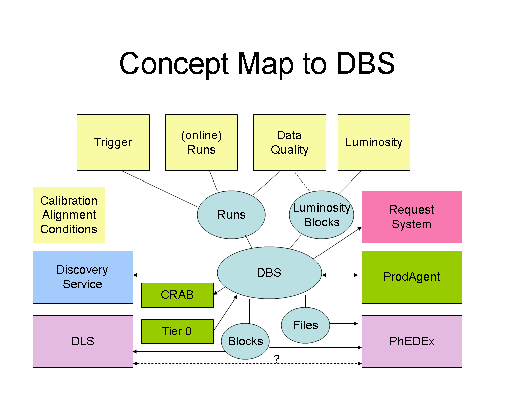
\includegraphics{figure/DBS-WS-DatabasesConceptMap-20060721.eps}}
    \caption{Concept diagram for DBS within CMS.}
    \label{fig:dbs-context-diagram}
  \end{center}
\end{figure} 

(Assignment: Lee will fill this in)

\section{Tasks and Use Cases from the  Workshop}

During the Cornell Workshop we compiled a list of 51 items to be followed up in our work to design the DBS system. There are several categories for the items and we have characterized them here as 1) use cases to be further expanded, 2) design requirement, 3) relationship with other subsystem in Data Management, 4) relationship within CMS at large.

\subsection{ Use cases to be further expanded}

   1.  (Assignment: Vijay)(use case, fermilab)Need to develop use case for publishing locally analyzed data to global scope - Fermilab

   2. (Assignment: Dan)(dbs)Fix a subset of a dataset due to problem found later, e.g. sqrt (-1) (changing does not affect the physics when it does not happen), calibration change. These are cases where only selected parts of the data need to be reprocessed, and then "blended" back in to the data set"

   3. (Assignment: Dan)(dbs)Need to track event processing failures in dbs, as reported by EDM in the job report run, event, reason for failure.

   4. (Assignment: Dan)(dbs)use pass ID to determine what data is interesting to analyze. Pass ID is equivalent to processing path name.

   5. (Assignment: Dan)(dbs)Allow for fruit salad mixing of data in a processed dataset.

   6. (dbs)Store filter information for each file (stream) for multi-output skimming


  14.(Assignment: Anzar) (dbs) Users need to store special data, such as log files or personal or group data.


  17. (review w/ ProdAgent, dbs)Merge and remapping requirements and use case. Is it really required (or advisable) that we get rid of intermediate files? Refer to SAM experience reported by Adam.

  19. (dbs)Who or which group created a particular set of data?

  21. (dbs, in progress)Schema review items: does family have any meaning in CMS? , Dans talk, review SAM schema, others.

  22. (use case-Drew,Lothar)Additions needed for CSA06: 1. find data based on application version, 2. link with DLS to find where data is.

  23. (use case) Need to go through analysis workflow (use cases) and determine additional API calls that will be needed.

  24. (Assignment: Dan)(use case-C.Jones)How is Analysis data set defined and how will it be used? Will it be static or dynamic (changes as new data is added or old removed)? Is there something like a snapshot? Are names prescribed for Anal DS, are they pre-fabed by physics groups or other admin policy. Can users create their own at will? What will UI look like, what is API required.?

  25. (dbs, FJR)Need way to have the set of tags (one for each subsystem) specifying calibration and alignment into DBS so it can be query-able. (it is in the config file)

  26. (Assignment: Anzar)(dbs) Introducing data from out side official processing machinery, so-called offroad data"

  27. (Assignment: Anzar)(usecase-?)Private and semi-private data sharing. How can you share data with colleagues at other institutions before it is ready for global scope publication.


Usecase: Introducing off-road data into DBS, produced outside official production


The main function of DBS will be to register available files and associated meta data. The data should preferably be defined by Framework Job Reports. DBS can provide explicit tools to process FJRs, extract required metadata and register files into DBS database.In case FJRs are not available or possible and it is still desired to register such files, DBS will provide a set of API calls that can be built into a custom tool for registration of such data files. There should be sufficient metadata available for the data to be registered into DBS. The off-road data can only be added by explicit privileges granted to certain people for this purpose. If produced data has parentage relationship to already existing data in DBS, it will be very highly recommended that DBS machinery ((local-global DBS) is used to produce and register such data. Also in this case proper parentage relationships will need to be registered.

We can have a set of DBS standalone tools, that generate "Data catalogs" as part of Data production in private environments, if producing FJRs is impossible, and then use these "Data Catalogs" to populate Local/Global scope DBS instances. Sites/People will be advised to use these cataloging tools as they write their job scripts. In some cases, we can have "translation" mechanisms from existing information to DBS Datacatalog format.


Usecase: Publication of Private Data before its Publication into Global scope DBS

One possible approach is to have a Local DBS setup at the site where private data is produced. Or use one of the nearest Local sites publish this data. The Local DBS instances could also have set of discovery tools associated with them. In this way Local DBS instances will have their own visibility. We could add a Status to Datasets/Files as "Promoted" or "Exported to Global" to identify which datasets are known by Global DBS. Secondly for a very short scope data production, Data Catalogs could be generated.




  28. (Assignment: Lee)(dbs)Getting runs into DBS, need DBS to have relation to luminosity block information.


  32. (dbs,FJR) Data tier is defined well enough to know what objects are in it. Some concern that this will change. How can we store the branch information from the FJR in a useful way? How will it be queried?

  33. (dbs) it is not correct to define parentage between processed datasets as some child data may be missing. Better to define at the file level.

  34. (dbs, some assumptions to clear up)Need way to select individual events from a particular tier given run/event.


  37. (dbs,FJR)The FJR should contain as much as possible of the information that is recorded in DBS.


  42. (?) Explore use of defaults for data specification [e.g. do not make people say 'AOD' since that is the most requested]

  43. (need more inout)How is DBS used for Online? what might DBS Track?
         1. Laser data
         2. alignment stuff
         3. express stream
         4. dedicated calibration runs
         5. Physics data> ==> Does DBS begin before or after repacking? << big issue. 


  44. (Assignment: Drew) (use case) How is DBS used for Tier 0?
         1. Reconstruction
         2. Tracking calibration and alignment output data 

  45. (Assignment: Drew)(use case) How is DBS used in Tier1:
         1. Re-reconstruction
         2. skimming 

  46. (Assignment: Drew)(use case) How is DBS used in Tier 2?
         1. MC Production
         2. Data analysis 

  47. (Assignment: Anzar)(usecase) How might DBS be employed for MTCC and Test Beam data?
         1. If a run table is added thenthis type of data could be added
         2. Under no pressure to make this work on a short time scale, but can use run for existing data to load the DBS catalog.
         3. Would be useful experience for the DBS system and good interaction form physicists. 

  
50. {Assignment: Valentin, in section on data discovery)(use cases) Data Discovery use cases and what should be available for discovery (Need subgroup to further explore this):
         1. detector experts looking at detector problems, Range of data (run range) with certain conditions, bad detector component, special trigger.
         2. What Physics meta data is needed to be related to datasets? Is it good enough to have 'simple' trigger name or all details of trigger needed? What high-level query-able things needed to store to find data? We need to make 'synthesized' easy to query versions AND allow full physics physics metadata discovery. 

  51. (dbs) From schema discussion:
         1. Three main concepts (more when have pictures of notes):
               a. Files
               b. Processings
               c. Datasets 
         2. We see no need to continue the concept of event collections.
         3. Schema was discussed and sketched out at workshop. Anzar will enter and draw using druid. 


\subsection{Design requirement}

  10. (dbs)All copies of a physical file are lost. Must be able to mark the status as unavailable or lost. Needs to be reported to DLS, and PhEDEx also.

  15. (Requirement)(dbs)Group needs a way to specify "official" data sets or analysis datasets.

  16. (Requirement)(dbs)Primary datasets must be special and have special meta data or ability to link to other information that characterizes it.


  18. (Requirement)(dbs)Authentication and authorization for DBS API

 new. Status flags for files, what else?

\subsection{Relationship with other subsystems in Technical Project}
   7. (dbs, need more info)support for pileup input datasets/files.

  11. (ReqSys?)Need a way to specify and submit processing requests for MC generation, and general data processing.

  12. (ProdAgent)Recovery of files that were not processed due to input failures, or high error rates in application.

  13. (ProdAgent)Recovery of data lost after processed. Outfile is lost 1. before entered into DBS, or 2. after entered in DBS.

  20. (?)Naming convention for processed dataset. Can this be automated.

  39. (ReqSys?-Giulio, dbs-fnal)Use cases for the data processing request system for both MC and real physics data processing. What is the overlap between the request system and DBS? DBS and the Request system share discovery of 'applications' (i.e. the configuration). It is assumed this sharing will not be needed for CSA06 but should be understood for the final system.


  35. (ProdAgent, dbs, Valentin)Need way to track, monitor, record usage patterns of the data access. Way to study history of data access. 

Here are the contact points between ProdAgent and DBS:
\begin{enumerate}
\item DBSComponent
\begin{itemize}
\item Creates Datasets   (both merge and processing)
\item Populates Datasets  (both merge and processing)
\end{itemize}

\item MergeSensor
\begin{itemize}
\item  Watches Datasets in polling mode
\item Retrieves fileblock information, generates merge jobs when sufficient data is present
\end{itemize}

\item PhEDExComponent
\begin{itemize}
\item  Queries DBS for fileblocks for an entire dataset for PhEDEx injection
\end{itemize}

\end{enumerate}


Other uses (not yet implemented but most likely will be)
\begin{itemize}
\item Remap Merge file parents to processing file parents upon completion of a merge job (DBS Component)
\item Validation/Invalidation of files in DBS
\end{itemize}
note: FJR shows which branches were used. probably want to dump FJR and logs in to archive, could be DBS. 


  40. (ReqSys?-Giulio) Confusion about meaning of payload and workflow in MC request system [Guillio needs to make a glossary that synchs up with the DBS jargon].

  41. (ReqSys?, dbs Gulio,Pete,Lee)The Request System and DBS are related but Peter thinks should be 'decoupled'. It seems possible and useful to link up the parameter set discovery system of the two in the long term. Not needed for CSA06.


\subsection{Relationship within CMS at large}
   8. (use case-?)data quality information. What level of granularity? run, luminosity block, event?

   9. (dbs, use case-?)Must be able to track luminosity for analysis dataset. Run over N luminosity blocks, some fail, some pass. How to integrate luminosity for all data used.

  29. (?)Need to have LFN naming convention.

  30. (use case, need more input) High level trigger information in DBS based on trigger mask, or trigger object, so can discover data based on trigger.

  31. (use case, need more input)Luminosity information stored in DBS? This information may change with time. Could have lumi block ranges and get luminosity from lumi DB.


  36. (dbs, need more input) How is file block name handled when published local to global scope DBS. Are files within the file block rearranged. Are more block attributes needed?

  38. (use case-?)What is the software environment an analysis user will be using while in the local scope? Who moves data and DBS info about the data from local to public scope and how is it accomplished? What is the software setup, configuration, and what tools are needed? What authentication and authorization is needed for this?

  48. (Assignment: Ian) (use case, dbs?) DBS/DLS/PheDex know about file/file block sizes
         1. How is this space 'assigned'/'allocated' at Tier-2 sites?
         2. Need tools to determine how disk (resources?) are used by "groups" in CMS?
         3. detail: Need to have concept of ownership (grolup/user) in either DBS or DLS
         4. research: map how people running jobs work within the constraints of the existing system (how do they deal with disk allocations, and stepping on one another's resources?) 

49. (need to present to other cms db players - Lee) Concept map for DBS and how it relates to other event and non-event data repositories. (DLS/DBS, conditions DB, trigger DB, luminosity DB, et cetera.

\section{Datasets and Processing}

\subsection{Physics Model Versus Storage Model}
This section discusses the CMS data model for real data, stressing the parts relevant to the DBS. The data model is a matter of physics, and we show here how it relates to CMS concepts of file storage.

This experiment will divide the continuous process of taking data into arbitrary runs. During those runs, calibration data for beam luminosity are recorded over time periods called lumi sections, or lumi blocks. We label the measurement made by the readout as an event, and a physicist would think of sets of those events as a lumi section or run. The last use of these names refers to their storage on disk, in bytes. Here we include files and file blocks, but a lumi section refers to the set of bytes which store the event data from a lumi section timespan.
\begin{figure}[hbtp]
  \begin{center}
    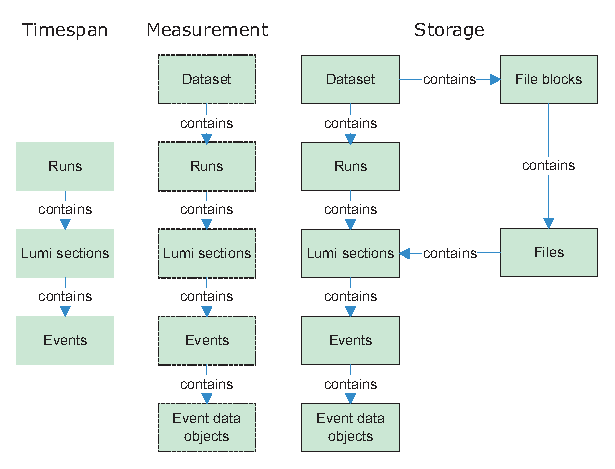
\includegraphics{figure/dataset_contains}
    \caption{The CMS data management system uses timespans to label storage of sets of events. We expect that a dataset will contain all data from a given run, but the important division for physics is the lumi section. For this discussion, solid lines show the storage model and dotted lines the physics model.}
    % To make eps from Visio, save as WMF. Open in Illustrator and save eps and pdf.
    % Include fonts. Use Acrobat full version to trim the pdf page.
    \label{fig:dscontains}
  \end{center}
\end{figure}
Note in Fig.~\ref{fig:dscontains} that the Dataset contains runs but runs do not necessarily contain file blocks. For data coming from the HLT, it would be natural to break file blocks on run boundaries, so runs may contain datasets in production, but later datasets are not guaranteed to contain runs. Processing under the SW Framework and ROOT does not have a concept of runs. They are just a convenience to mark larger time spans than lumi sections, so this should not affect processing.

A goal of the CMS Data Management System (DMS) is to allow physicists to interact with data in terms of the physics data model and think less about file storage. Let's examine some of what is known about the data management system and how it relates to models of the data and the analysis process.

When a physicist runs a job, the DBS records the files input, the process's application, and tracked parameters (those relevant to what algorithm is run). A simple picture is in Fig.~\ref{fig:dsprocess}.
\begin{figure}[hbtp]
  \begin{center}
    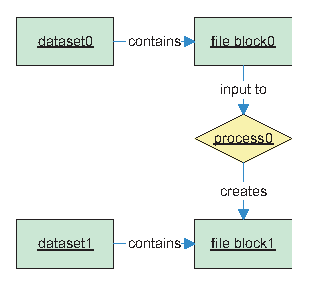
\includegraphics{figure/process_simple}
    \caption{The names in this diagram have underscores because it shows the relationship among instances of file blocks and processes instead of showing the relationship among the concepts, as in Fig.~\ref{fig:dscontains}. There can be no quibbling that a job accepts file blocks as input and produces file blocks.}
    \label{fig:dsprocess}
  \end{center}
\end{figure}
The file blocks into or out of a job can belong to one or more datasets, with this model, unless policy forbids it. Because most jobs for this experiment process data event-by-event, each event is labeled with an event id. Each lumi section also has an id. We refer to the events in the output dataset by the same event id as those in the input. The same goes for lumi sections. You might think of these, instead, as instances of the event or lumi section. How does the data in the dataset correspond to a physics analysis picture of the data model?

If we think of two analysis steps, where the second algorithm uses some of the same input as the first, we might picture it as in Fig.~\ref{fig:dsdoubleinput}. There is no copying of data, but the second algorithm reads two sets of file blocks.
\begin{figure}[hbtp]
  \begin{center}
    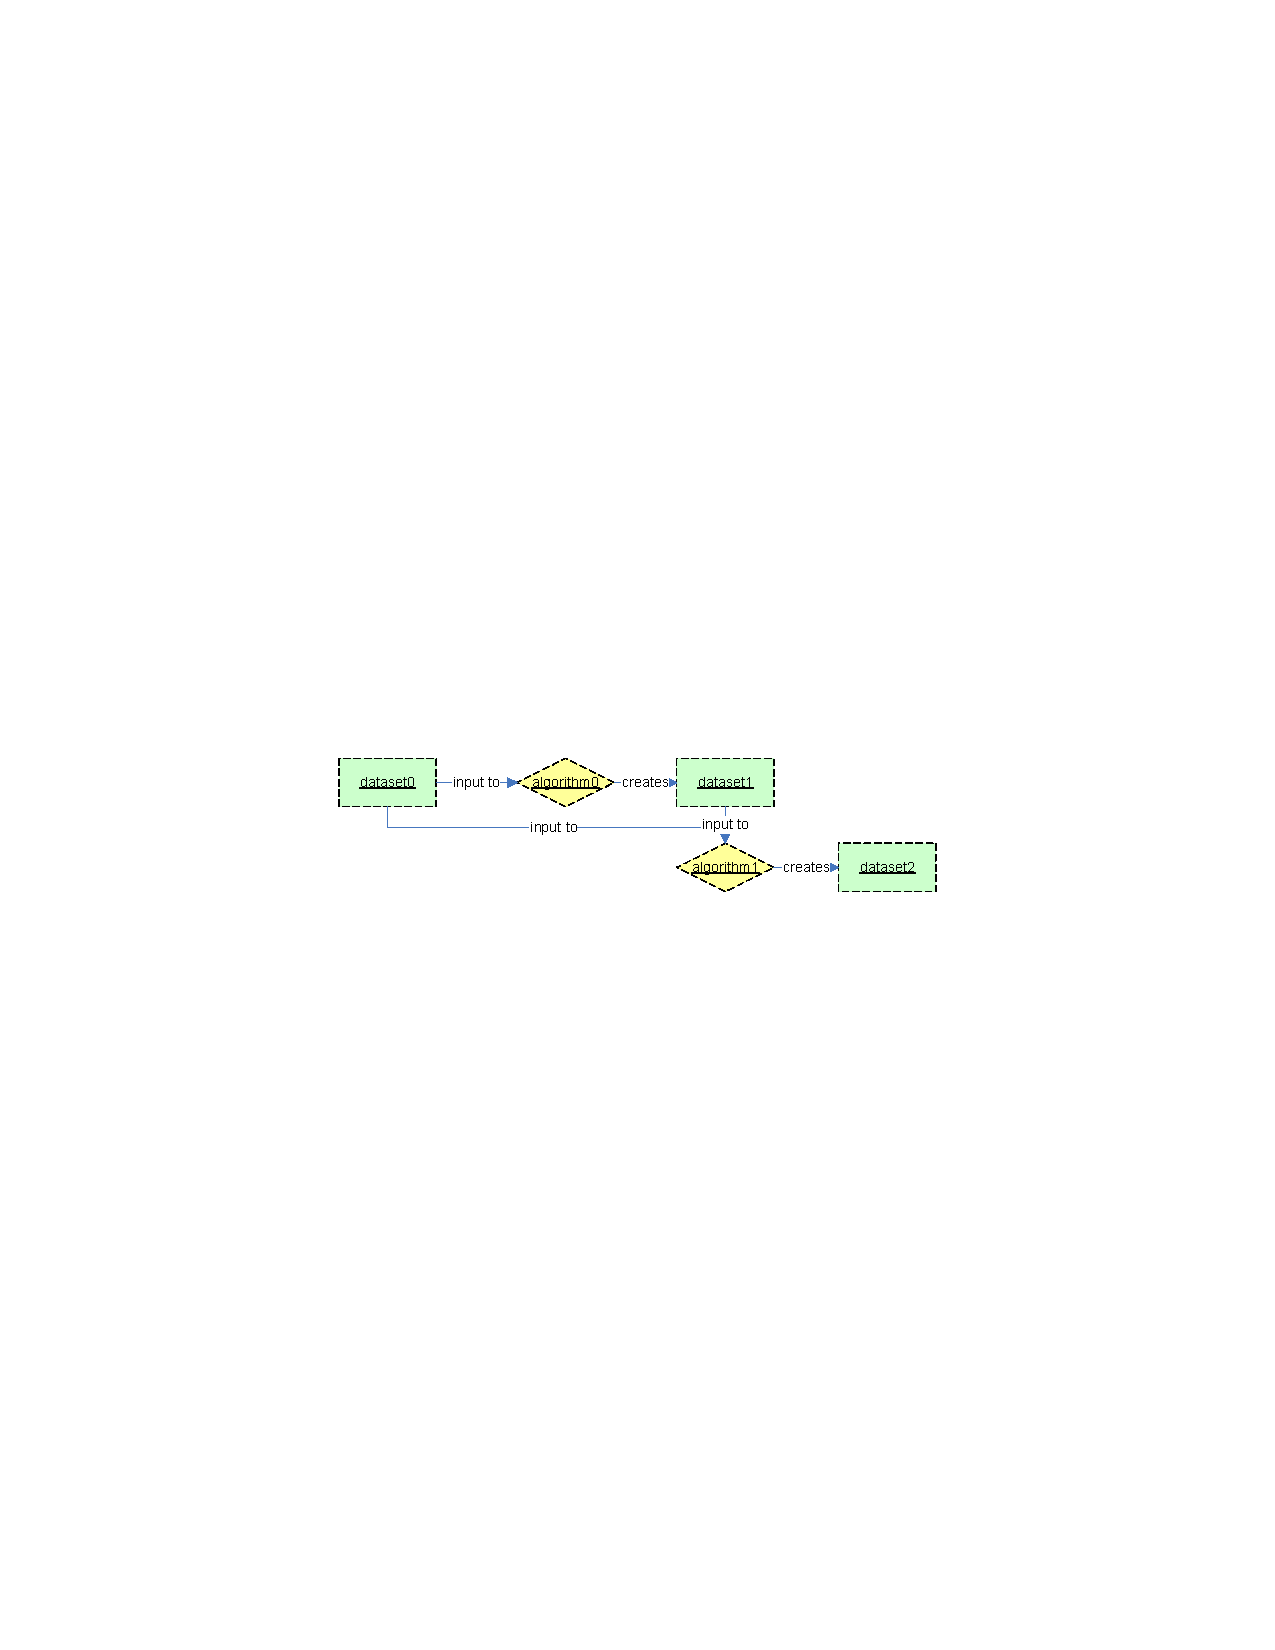
\includegraphics{figure/double_copy}
    \caption{This is a fictitious example of analysis where there is no copying of data.}
    \label{fig:dsdoubleinput}
  \end{center}
\end{figure}
This experiment often optimizes this process by copying some or all of the input data into the output, as shown in Fig.~\ref{fig:dscpforward}. There are still times a job will require more than one input dataset, but copying some input increases efficiency.
\begin{figure}[hbtp]
  \begin{center}
    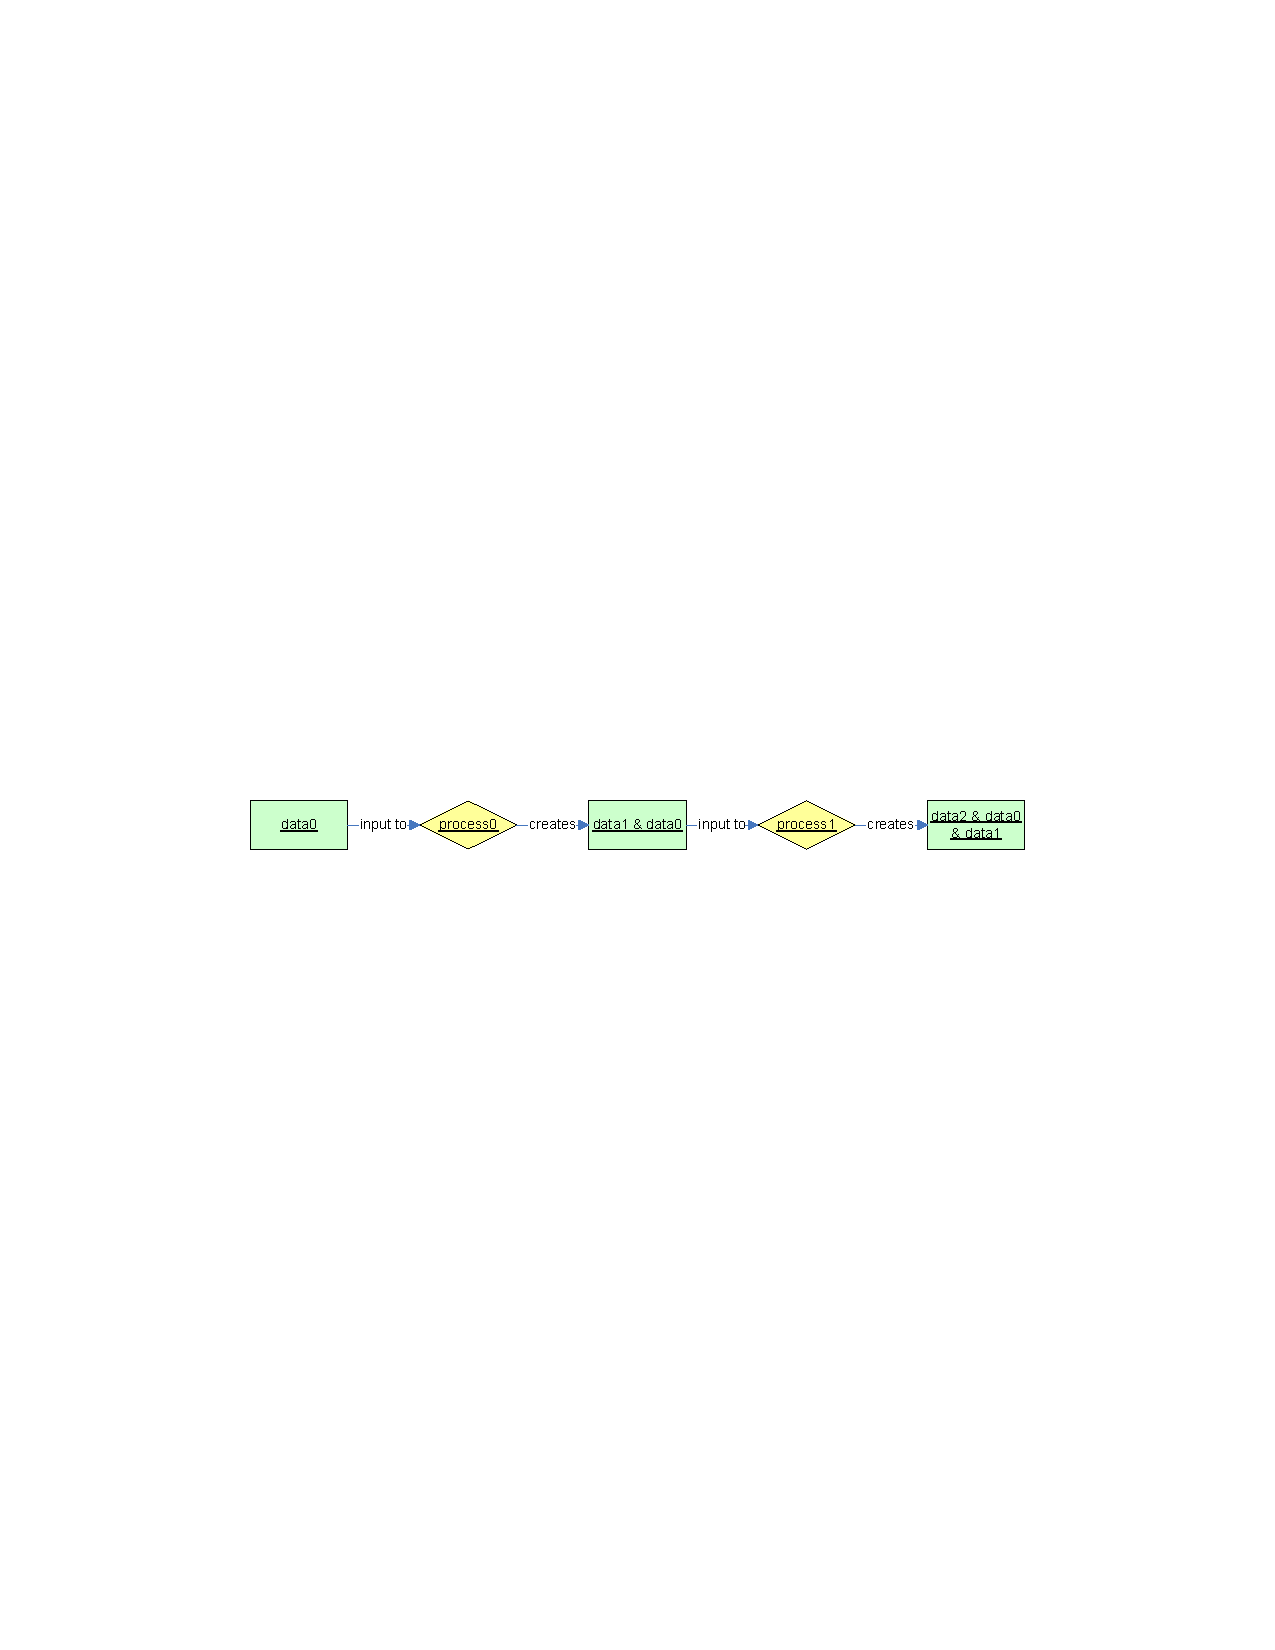
\includegraphics{figure/copy_forward}
    \caption{Processes often take all or part of the input dataset and copy it into the output dataset because later jobs will need the data.}
    \label{fig:dscpforward}
  \end{center}
\end{figure}
There are two ways one could combine data in an output set of file blocks. One is to combine it on the event level
\begin{quote}
  evt0 \{ data0, data1 \} evt1 \{ data0, data1\},
\end{quote}
and the other is to keep event storage from one processing step separate from event storage for the other processing step
\begin{quote}
  data0 \{ evt0, evt1 \} data1 \{ evt0, evt1 \}.
\end{quote}
This experiment does both. Data objects within an event define the data tier for that bit of event storage. A file block containing events of a certain data tier is said to have that data tier, but a dataset may contain other file blocks whose events contain a different subset of the analysis result in their events. Fig.~\ref{fig:dsdstiers} shows a dataset which is in three tiers at the same time. Because AOD data objects are stored in separate file blocks, a job can request those files separately without transferring the larger RAW and RECO data objects.
\begin{figure}[hbtp]
  \begin{center}
    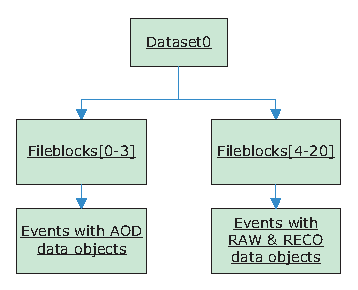
\includegraphics{figure/dataset_tiers}
    \caption{A dataset is composed of file blocks. All events in a file block must contain the same types of data objects, so we say they have the same data tier. The resulting dataset is therefore in the AOD, RAW, and RECO tiers.}
    \label{fig:dsdstiers}
  \end{center}
\end{figure}

Fig.~\ref{fig:dsalgselect} shows how a physicist might refine the model from Fig.~\ref{fig:dsdoubleinput}. It just shows that selecting a data tier slices a dataset and that analysis steps may copy some data to the output. This poses a small wrinkle
\begin{figure}[hbtp]
  \begin{center}
    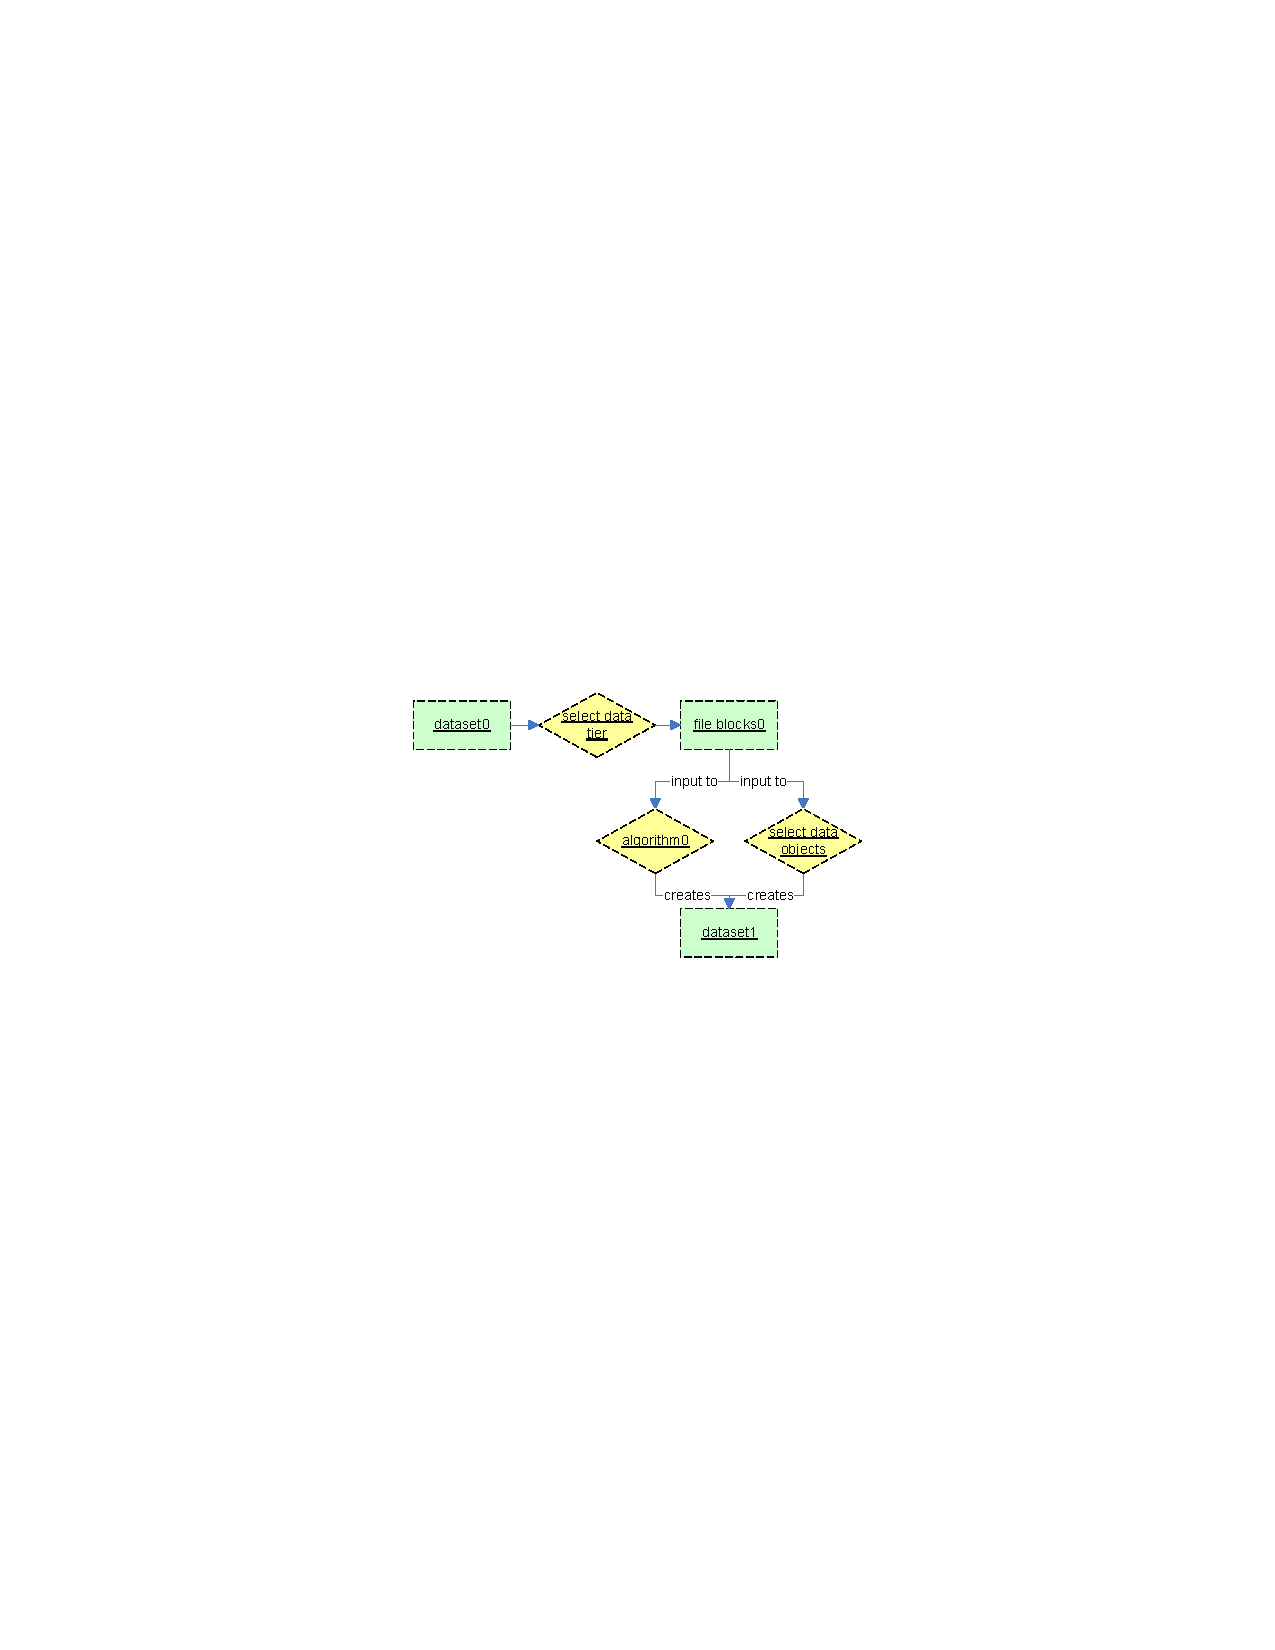
\includegraphics{figure/algorithm_select}
    \caption{For CMS DBS, the physicist will choose a processed dataset both by name and by data tier. Selecting a dataset by data tier effectively selects only those file blocks of the dataset that contain events with the desired data objects. In addition, the complication of copying data from input to output makes a slight change in how a physicist might think of the analysis step.}
    \label{fig:dsalgselect}
  \end{center}
\end{figure}
for questions about whether a particular dataset is a descendant of another dataset. From Fig.~\ref{fig:dsprocess} we have a straightforward way to determine if a file block is a descendant of another file block. Once we copy forward data objects, and possibly whole file blocks, we introduce ancestors to file blocks which are not correct from a physics analysis perspective. It is, however, probably not a big deal.

\subsection{Multiple Processing Steps May Be Done At Once}
cmsRun is capable of performing several processing steps at once. For instance, sometimes the GEN, SIM, and DIGI steps are done in one job. That means the two graphs in Fig.~\ref{fig:dstwostep} could produce file blocks that are part of the same dataset. Their explicit ancestor tree would differ, but they were processed with the same algorithm. For the purposes of constructing the dataset, this would not matter much. The input configuration file specifies the name of the output dataset, and the DBS will publish the output file blocks from both jobs in the same dataset.
\begin{figure}[hbtp]
  \begin{center}
    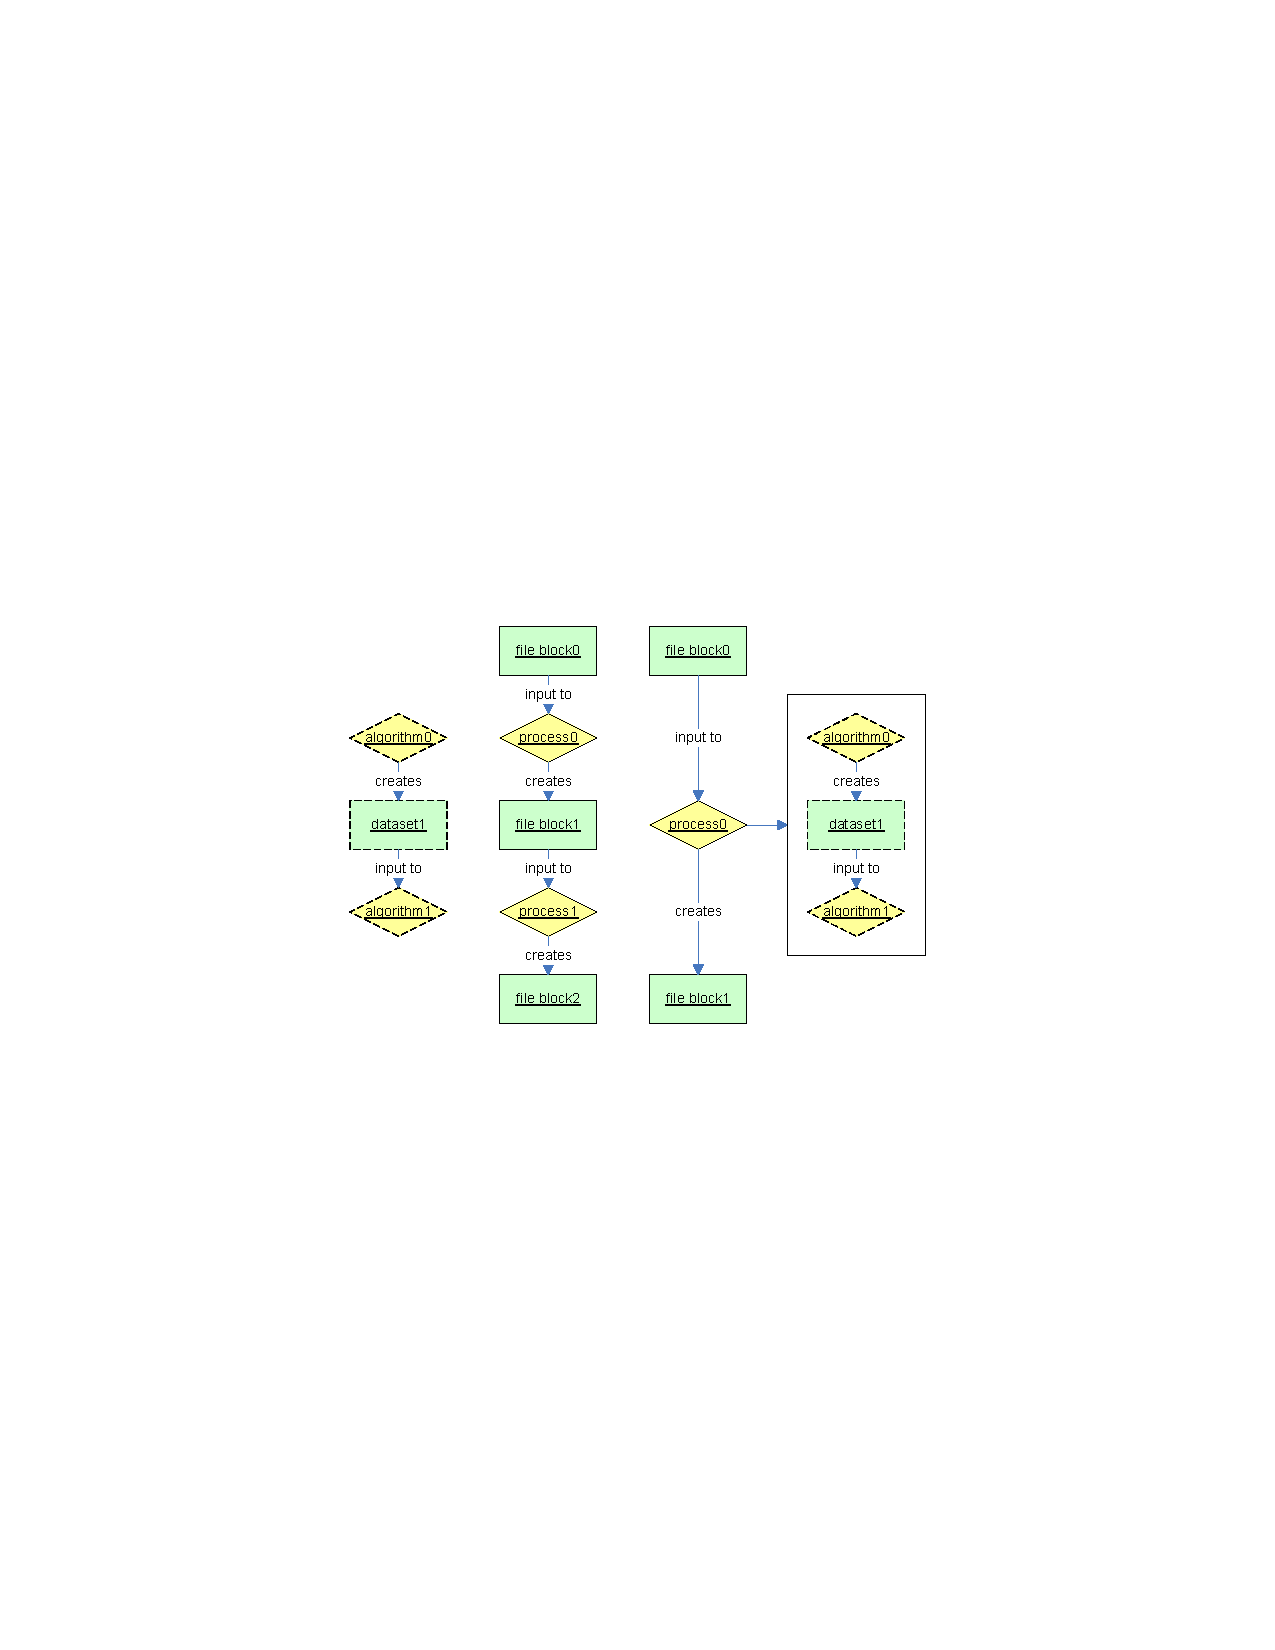
\includegraphics{figure/process_twostep}
    \caption{Two different processing histories can produce the identical results. The single process on the right is executing the same two algorithms as the one on the left. For whom is it important to identify these histories expressing the same physics?}
    \label{fig:dstwostep}
  \end{center}
\end{figure}

If two people wanted to compare the processing of their results, they would look at the ancestor tree and figure out that the steps used identical physics. As long as that can be done by eye, it should not matter much whether the processing was done in one or two steps, but there are hundreds of possible variations in processing for each step, so we will likely want to automate the comparison of provenance for two analysis results.

The file blocks resulting from one or two processing steps would contain slightly different metadata. cmsRun and ROOT record which process created an event data object, so some event data objects would be marked with only one process name versus two. This could matter for the next analysis step on the output dataset because ROOT uses the process name as part of how it specifies input event data objects. cmsRun, with its EDM, reads back to find the required results, so it would not have difficulties.

\subsection{Datasets May Contain Duplicate Events}\label{duplicate_events}
If subsequent jobs can add to the same dataset, it is possible for them to add file blocks which duplicate events. Because jobs process data in sets of lumi sections, that means there would be two or more lumi sections with the same id. This is shown in Fig.~\ref{fig:dstwolumi}.
\begin{figure}[hbtp]
  \begin{center}
    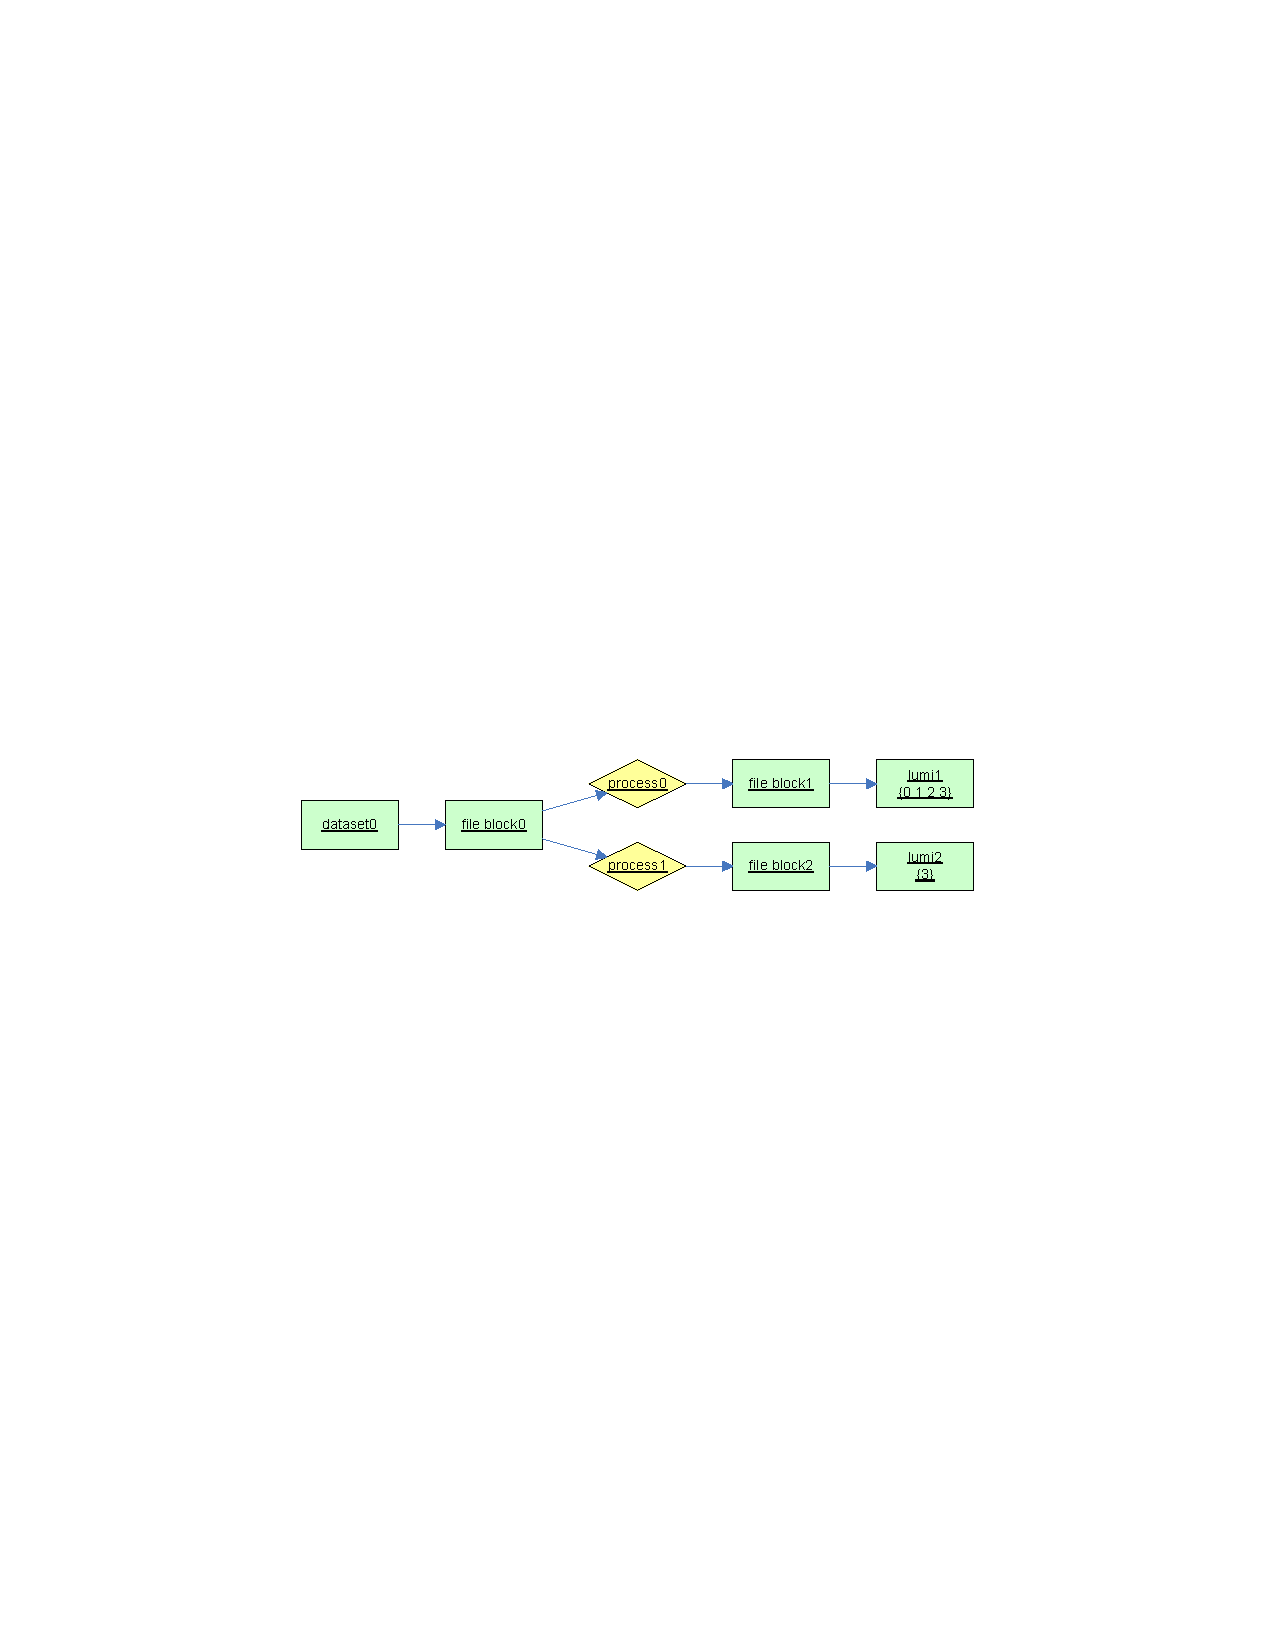
\includegraphics{figure/duplicate_lumi}
    \caption{Processed datasets can contain duplicate events. There must be some way to find out which ones to use for later analysis.}
    \label{fig:dstwolumi}
  \end{center}
\end{figure}
There are good reasons to do processing in many steps. If a job tends to die, it can be more efficient to split that job. If one job had error only for a few events, such as a $\sqrt{-1}$ error, a second job might fix that problem without significant change to the algorithm. It is even possible for a job to fail because of hardware errors, in which case the second job will have no algorithmic differences from the first. That means there will be no changes to the tracked parameters or to the application name and version.

How then do you identify which lumi section is which? You could go into the first file block and mark lumi sections as bad, but we tend to think of files as inviolate once written. They may already have been spirited to far shores by \phedex. You cannot mark them by application version. What distinguishes those lumi sections is both the unique operating system process that calculated them and the unique file block in which they are stored. They would have to be tagged with one of these two.

For this experiment, files are inviolate once they are written. We cannot return to a file and mark lumi sections as bad. This information must be stored elsewhere, likely in the DBS.

\subsection{What is a Pass?}
This experiment would like to introduce to the data model the idea of a pass because it has been useful in previous experiments.
In order to support this idea in the storage model, we have to decide what similarities among datasets are important.
\begin{figure}[hbtp]
  \begin{center}
    
\includegraphics{figure/run_stream}
    \caption{Our basic idea of a pass is that we reprocess the same data. We may redo the data because we have improved cmsRun or because we have better conditions, but we would like to associate the new dataset with the old as a recommended substitute.}
    \label{fig:dsrunstream}
  \end{center}
\end{figure}
\subsubsection{Pass as Re-Running With Newer Algorithm}
\begin{figure}[hbtp]
  \begin{center}
    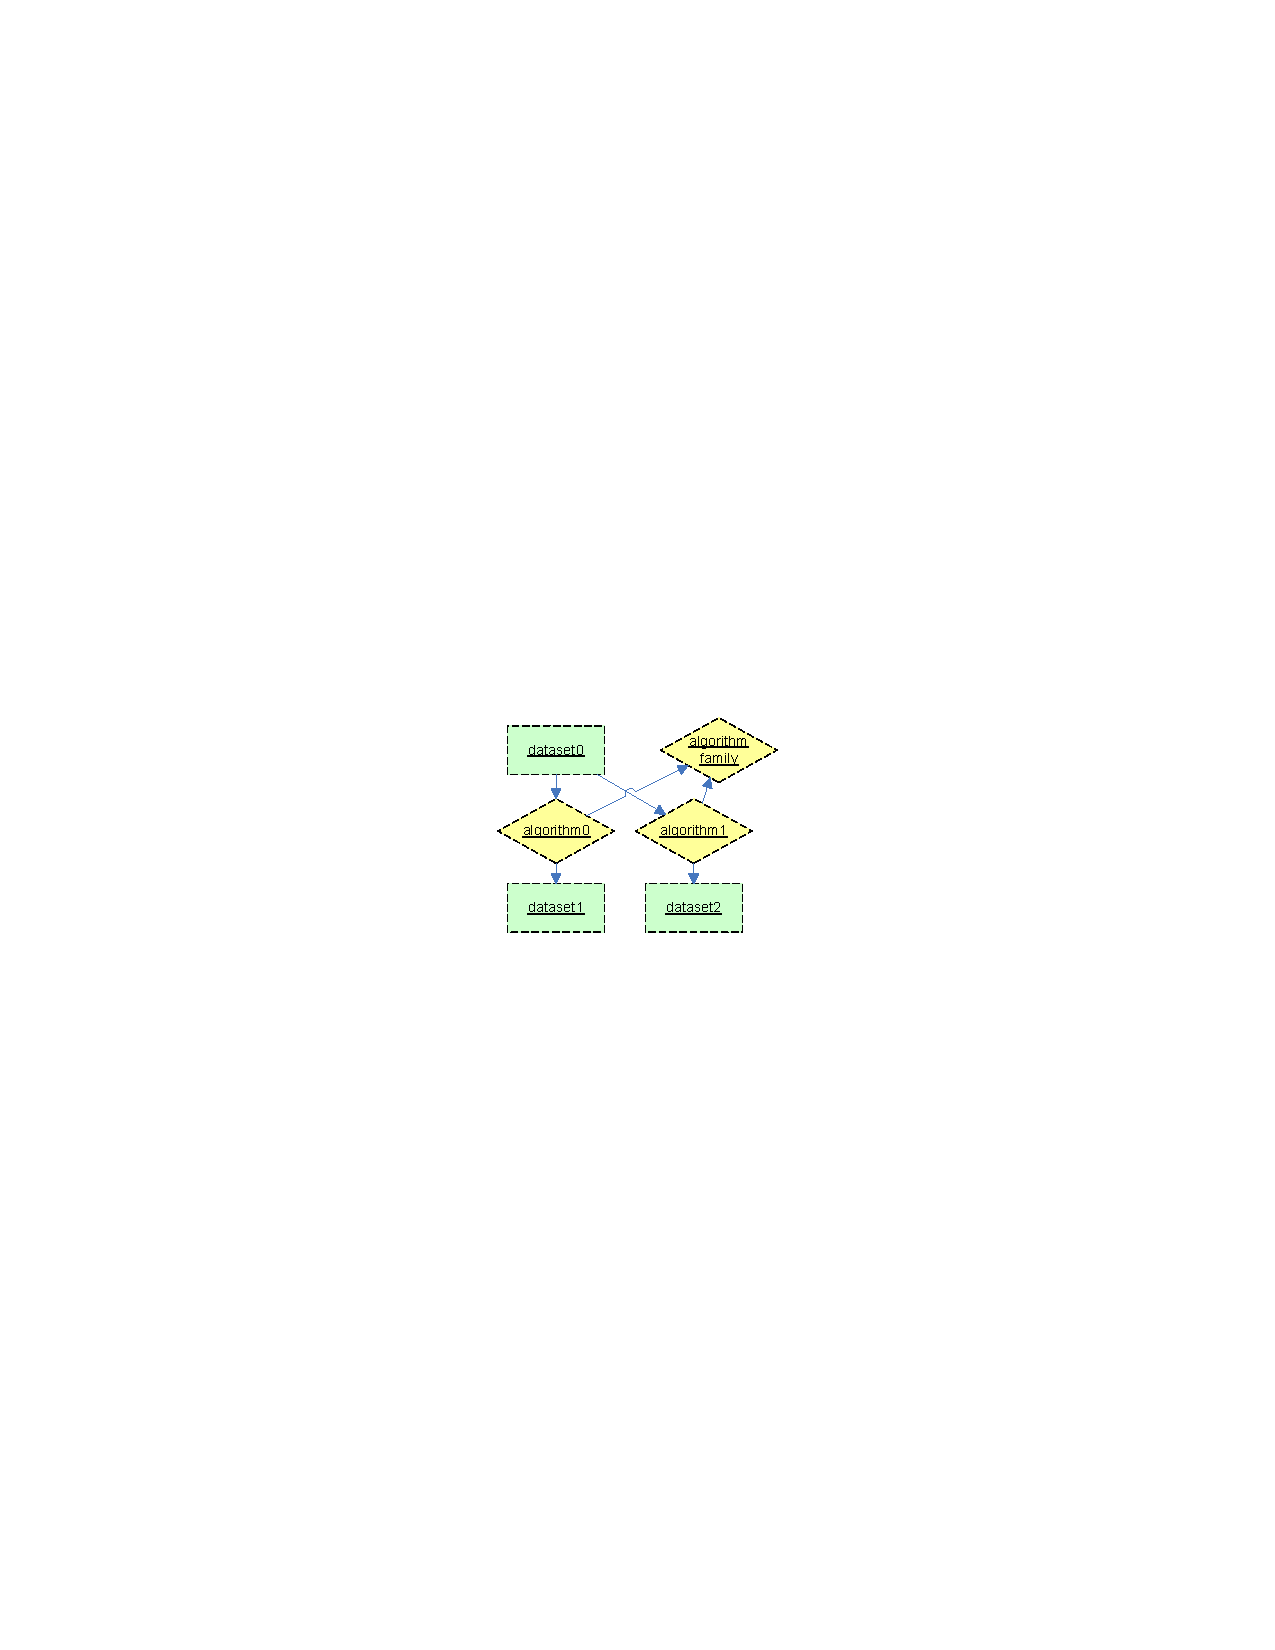
\includegraphics{figure/algorithm_pass}
    \caption{One idea of a pass is that two jobs executed algorithms similar enough that their resulting data has the same physics intent. The resulting datasets are then called passes of each other. The input data for the second job is either the same or a pass-of the original input data.}
    \label{fig:dsalgpass}
  \end{center}
\end{figure}
One idea of a pass is that a newer version of cmsRun, using the same input parameters and conditions, would produce a new dataset that is, hopefully, an improvement on the old one. Here, a pass of a dataset is a dataset whose processing history was sufficiently similar that we might substitute the newer for the older when doing further analysis. This is shown in Fig.~\ref{fig:dsalgpass}. If we wanted the physicists' user interface to reflect this concept, then reprocessing a dataset, for instance re-RECO, would produce a new dataset of the same name but different pass id. At least, the DBS could identify that a newer dataset with a different name is a pass of an older one. 

There isn't necessarily a way to automate identifying when two algorithms are passes of each other. Sometimes a change to a tracked parameter is a minor improvement on the algorithm, but other times it is an important modification or an experiment.

Several possible schemas for the DBS have, at times, included entries for application families. These application families group applications as similar. This is not a sufficient way to capture the algorithm family described above because, for ROOT and cmsRun, the algorithm depends upon not only the application but also the configuration file's tracked parameters and the conditions those tracked parameters specify.
\begin{figure}[hbtp]
  \begin{center}
    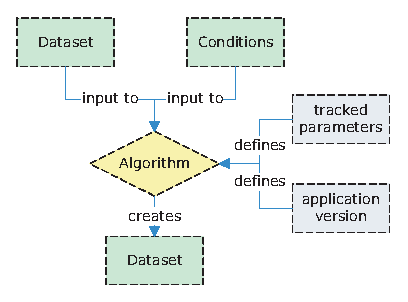
\includegraphics{figure/simple_dataset}
    \caption{An application is not the same thing as an algorithm, especially for cmsRun and ROOT which load different modules depending on their configuration files. Knowing that two jobs were processed by cmsRun does not imply they were processed with the same algorithm.}
    \label{fig:dssimpleds}
  \end{center}
\end{figure}

\subsubsection{Pass as a Conditions Version}
Another idea of a pass, shown in Fig.~\ref{fig:dscondpass}, is that all datasets processed with the same version of the algorithm but different versions of the conditions database are of the same pass.
\begin{figure}[hbtp]
  \begin{center}
    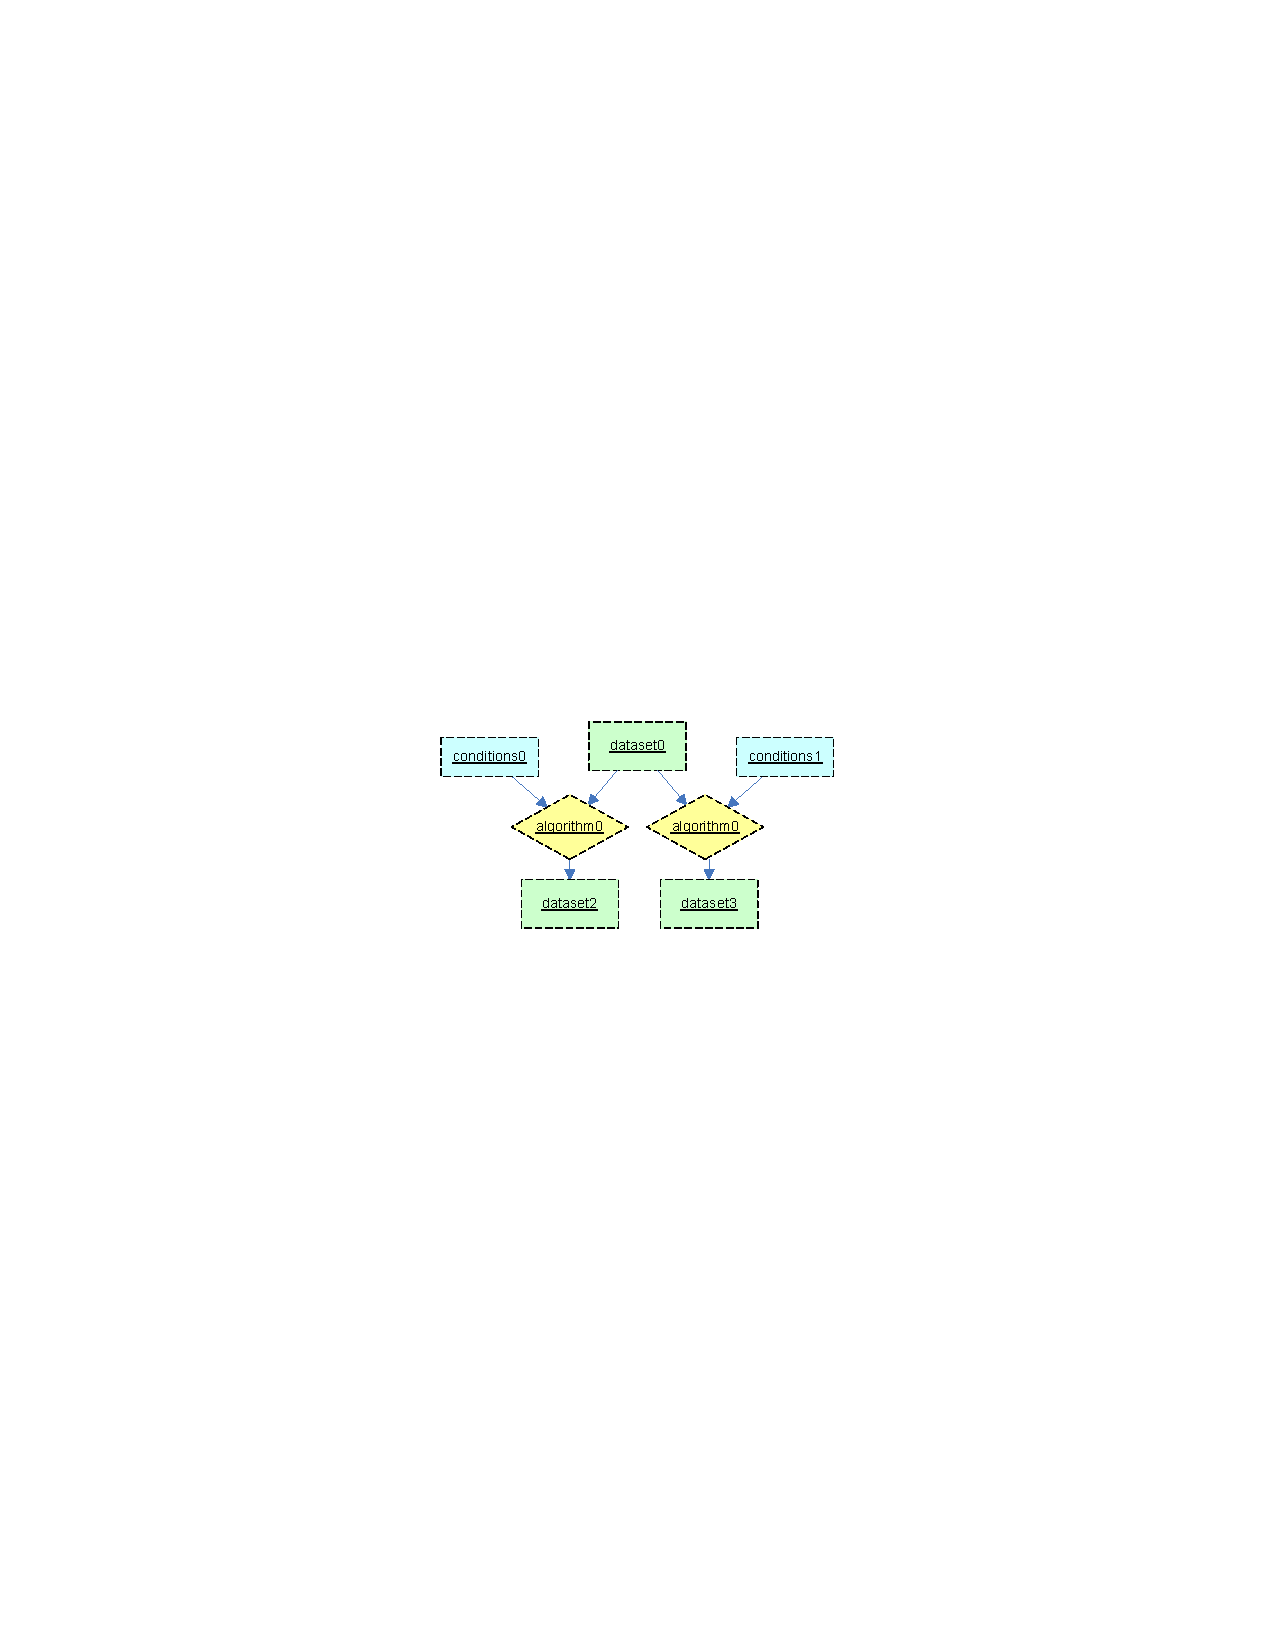
\includegraphics{figure/conditions_pass}
    \caption{This definition of a pass was used in CDF. Every dataset processed with the same algorithm but different conditions was considered to be passes of each other.}
    \label{fig:dscondpass}
  \end{center}
\end{figure}
This version could be automated. Datasets would not necessarily have consecutive pass ids, but they don't have to be consecutive to label them as passes of each other.

\subsubsection{Pass by Fiat on Analysis Datasets}
A least idea of a pass could be that an analysis dataset could be a pass of a previous analysis dataset. Analysis datasets are snapshots of processed datasets, and they should never change. That means they are a list of file blocks, specifying which lumi sections to use from those file blocks in order to rule out duplicate events. Because analysis datasets are defined by fiat, by the arbitrary decision of a data quality group, later passes of analysis datasets could be defined the same way. There need be no algorithmic or provenance similarity to the previous analysis dataset as long as the physics intent of the dataset is similar.

For a physicist, whether an analysis dataset is a pass of another analysis dataset has little to do with the processing history. It is an assertion that the newer dataset can be substituted for the older one in further processing.

\subsubsection{Corrections May Not Be a Pass}
When there is a small algorithm error which affects only a few events, it can be convenient to fix the error and re-run only the affected events, then tuck them into the original dataset. We discussed in section~\ref{duplicate_events} how a dataset might contain two instances of the same lumi section. Is this a new pass, and how might we implement it?

Correcting an algorithm, even by correcting detector conditions for a small set of events, does change the output. The set of events processed with the old algorithm are one pass, and the newer pass is the set of events processed with the new algorithm plus those old ones which would not have changed were they to be processed by the newer algorithm.

What if we want to make both the old and new passes available to the physicist? How does a physicist expect to find a new pass of a dataset? The simplest way is to find the new dataset with a new name. We may, possibly, implement passes such that the new dataset has the same name but different pass id. A further possibility is that the old pass of the data is available within the dataset, accessible as a list of deprecated lumi sections.

If we don't believe physicists will want to access the deprecated lumi sections from the first pass, then only the newer pass of data need be available, and it should be available by default. The deprecated lumi sections could be marked the same way that we mark lumi sections which contained other kinds of failures, such as CPU floating point problems.

\section{Discovery Questions To Fold In With Valentin's Section}

Relationships among datasets
\begin{itemize}
    \item ancestor/descendant of
    \item containment, subset/superset of
    \item pass-of, for algorithms, conditions, or analysis datasets
    \item skim-of, which is a special case of descendant
\end{itemize}
A skim is a dataset which reads event data and produces event data with no new event data objects.

Questions about a particular dataset
\begin{itemize}
    \item Size, luminosity, dates written, when accessed.
    \item Location of files relative to places where user can do processing.
    \item What is the HLT of the ancestor?
    \item What algorithm wrote this data and its ancestors? This may be answered best by both the application name and a list of products in the config file.
    \item What data objects are in this dataset? From which processing steps?
    \item What conditions were used as input to this dataset and ancestors?
    \item Has a data quality group approved any lumi sections in this dataset? or any lumi sections in an ancestor or descendant? Have any lumi sections from this dataset been included in an analysis dataset?
\end{itemize}

\section{Use Cases}
The primary actors for these usage narratives and use cases are often applications or services defined in the glossary, but the first round of usage narratives focuses on the actions of people. We define their roles here.
\begin{description}
\item[Backup Operator] Ensures DBS can be restored in case of failure.
\item[Collaboration Manager] Oversees a physics analysis effort at a Tier~1--5 site. Concerned with data integrity and security.
\item[Detector Expert] On site with the detector, this person is responsible for the quality of raw data.
\item[Physicist] A physicist analyzes detector data and its products in order to measure physics processes.
\item[Production Run Manager] This person initiates and monitors the processing of data.
\end{description}

There are some missing tools, as well. You might even believe these tools already exist, except that they have yet to receive cute names with intercapitalization.
\begin{description}
\item[Data Discovery Tool] This tool allows physicists to find which datasets express the physics of interest. It is currently a web page.
\item[Provenance Tool] This is an application which allows a person to create, modify, or delete data in the DBS.
\end{description}

\subsection{CSA06}

Several use cases for the upcoming CSA06 work are illustrated in Fig.~\ref{fig:csa06-use-cases-diagram} and described in this section. CSA06 will use Monte Carlo data to simulate real data from the detector. This data will pass through the HLT and all production steps, ending in several steps of physics analysis. The CSA06 test will use a version of the DBS and other tools current as of July 2006.
\begin{figure}[hbtp]
  \begin{center}
    \resizebox{0.8\textwidth}{!}{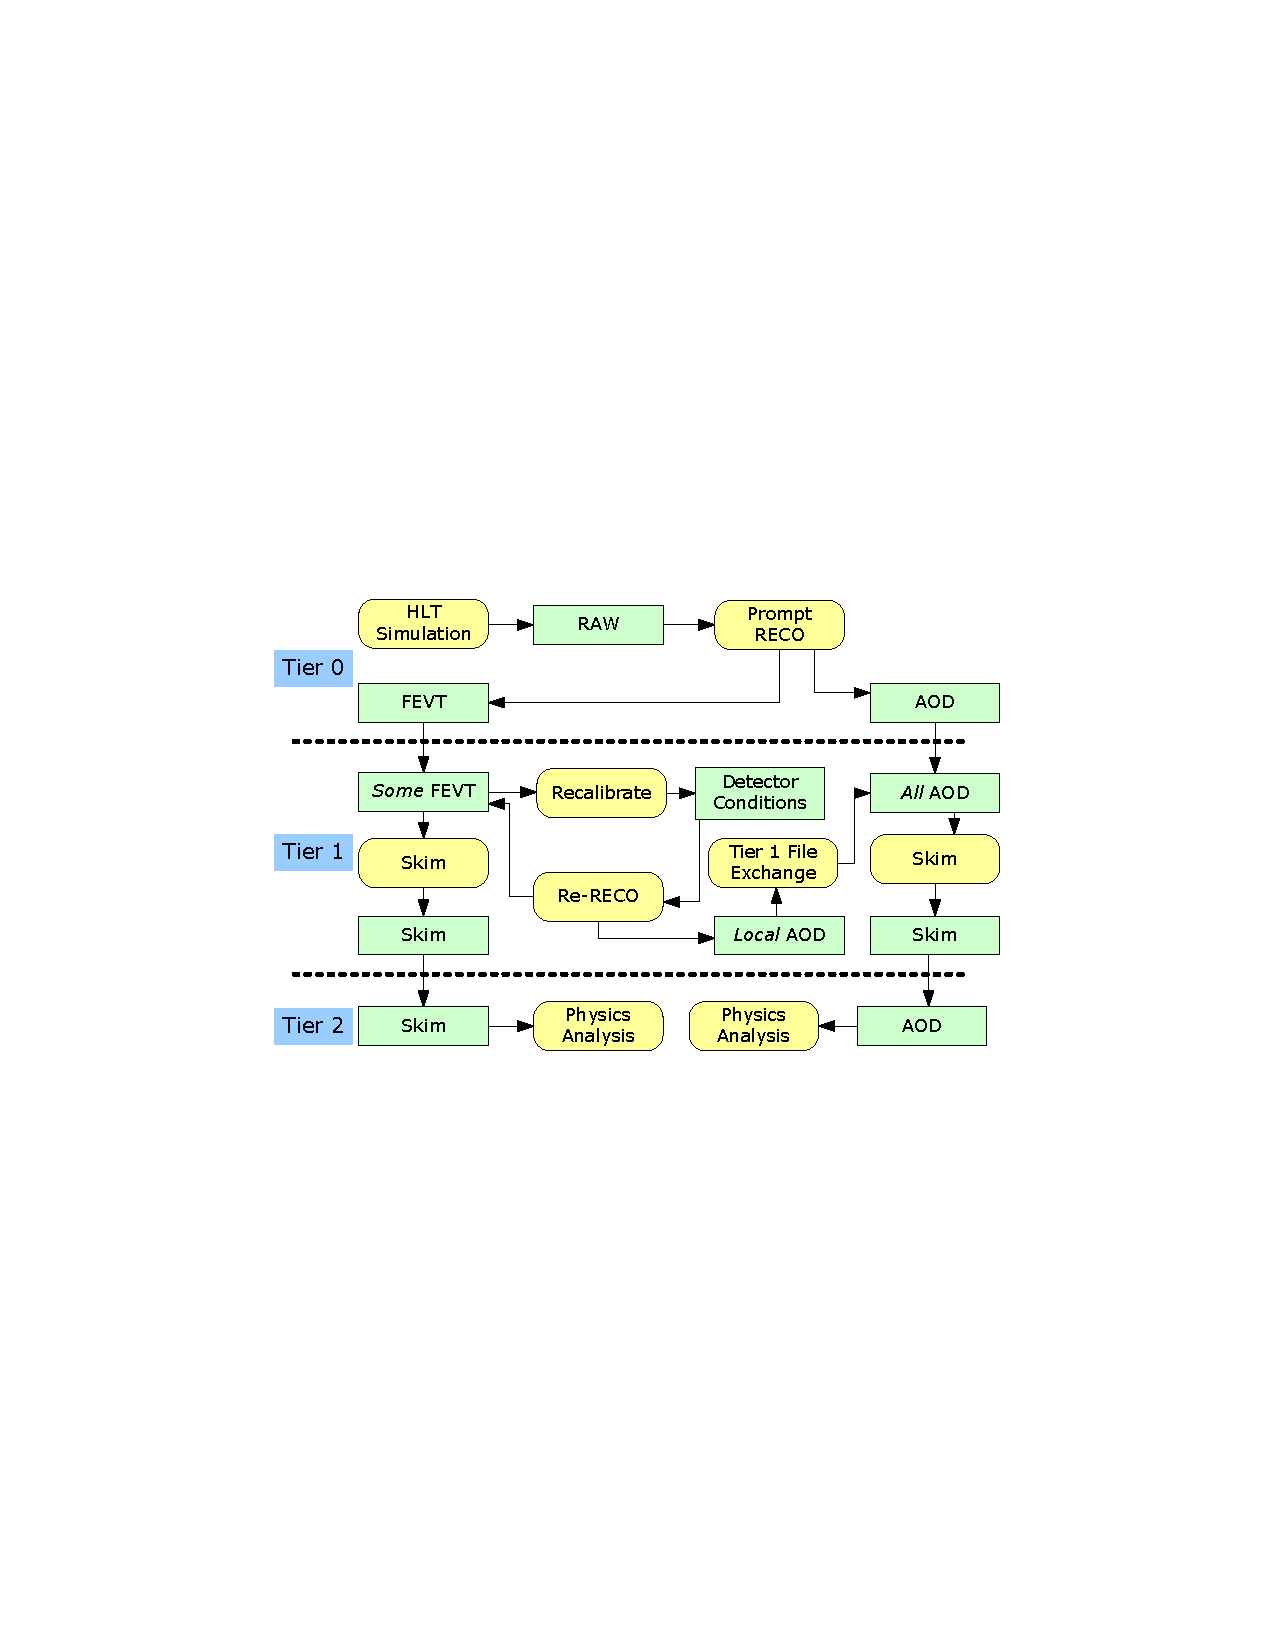
\includegraphics{figure/CSA06_use_cases_dfd}}
    \caption{This data flow diagram for CSA shows processing in yellow
    and products in green. \phedex performs transfers across data tiers
    and the ``Tier~1 File Exchange" of AOD among Tier~1 storage.}
    % To make eps from Visio, save as WMF. Open in Illustrator and save eps and pdf.
    % Include fonts. Use Acrobat full version to trim the pdf page.
    \label{fig:csa06-use-cases-diagram}
  \end{center}
\end{figure} 

We can write a usage narrative for most of the steps shown in Figure~\ref{fig:csa06-use-cases-diagram}. Because CSA06 is a simulation of what would be done with real data, it starts from the production of DAQ-RAW.

\begin{narrative}{Production Manager Creates Real HLT Data from MC Data}
Production Manager runs the HLT on a large dataset of MC Data. Production Manager uses Provenance Tool to put that data into the DBS. Only five million events go through the HLT from all of the MC data, and the DBS tracks these.
\end{narrative}

\begin{narrative}{Tony at Tier~0 Presents Raw Data from HLT\label{narr:tony0}}
Tony uses a set of scripts to process simulated HLT data. He asks a program to make file blocks from that data. He asks Provenance Tool to put that data into the DBS.  Tony gives tool Provenance Tool a list of information, which we will figure out below. Provenance Tool contacts the Global DBS to place correct processing history.

Does Tony know which primary dataset names to use? How are the primary datasets for real data managed at the Tier~0? How are primary datasets for MC handled?
\end{narrative}

\begin{narrative}{\phedex Transfers Data Among Facilities\label{narr:phedex}}
All of the places that the diagram shows a transfer, it is done by \phedex. Someone tells \phedex to look for a particular file in the DBS, and it will transfer that file. \phedex works by subscriptions, so a site can subscribe to receive every file block belonging to a particular primary dataset. Can \phedex transfer individual skims to Tier~2 sites for further processing?
\end{narrative}


\begin{narrative}{Alignment Person Recalibrates Using $Z$ to $\mu$-$\mu$ to Produce a New Version of Alignment\label{narr:recalib}}
Data Quality Expert polls Data Discovery Tool which shows a list of available datasets. He knows that he is looking for FEVT from CSA06 and that this FEVT data should be straight from the HLT, not reprocessed in any way. (Should be done at CAF, but not for CSA06.)

He submits the alignment job to CRAB or Prodagent. He specifies a subset of the total FEVT dataset. The recalibration job returns new detector conditions. He gives these detector conditions to \emph{someone\/} who places them into alignment database where they will be found by future RECO production. (It could be a job robot that runs this instead of Prodagent or CRAB. How do you insert new detector conditions? Do you need a new version of the software or configuration.)

The Data Quality Expert then asks Prodagent to create RECO and AOD from the RAW data within the FEVT. He already knows the exact dataset but may use a different subset than was used for recalibration. Prodagent performs this calibration and creates a new, partial set of FEVT and AOD.
\end{narrative}

\begin{narrative}{Physicist Tier~2 Creates Skim of Re-RECO at Tier~1\label{narr:skim2}}
Physicist looks for re-RECO data from a recalibration at Tier~1. (Will there be more than one?)
Finding that dataset, he asks which Tier~1 has that data. He puts some identifier for the dataset into a Prodagent job, along with the name of the Tier~1 on which to do processing. Prodagent creates the skim and registers it in the Global DBS.
\end{narrative}

\begin{narrative}{Physicist Tier~2 Runs Analysis Job}
Physicist has just created a skim of Tier~1 FEVT data from re-RECO. He needs to tell \phedex to transfer that data to his Tier 2 site. Then he tells CRAB to run that job.
\end{narrative}


\begin{narrative}{Physicist Tier~2 Runs Skim on One of Six Copies of AOD}
This is much like narrative~\ref{narr:skim2} except that the file type is AOD. He must perform a skim at a Tier~1, ask \phedex to transfer that skim to the Tier~2, and then process it.
\end{narrative}


\begin{narrative}{Production Manager Watches CSA06 Progress}\label{narr:csamanager}
Production Manager wants to see what data exists and what file blocks are transferred. They open a Data Discovery Tool. It queries the DBS for file existence and \phedex for file transfer rate. (Can \phedex tell you this? Would something else do it, like the DLS?)
\end{narrative}

\subsection{Data Discovery for CSA06}
From the usage narratives above, we can compile needs for data discovery.
\begin{itemize}
\item \phedex identifies a subset CSA06 FEVT data for transfer to Tier~1. (\ref{narr:phedex})
\item \phedex identifies CSA06 AOD data, whether produced by Tier~0 or Tier~1, and transfers it to particular Tier~1 facilities which subscribe to different trigger lines. (\ref{narr:phedex})
\item \phedex identifies a particular skim dataset, created by a Physicist, from Tier~1 to Tier~2. This can be either FEVT or AOD. (\ref{narr:phedex})
\item Data Quality Expert needs CSA06 FEVT data that is identifiable as coming straight from Tier~0. (\ref{narr:recalib})
\item Prodagent has to be able to find RAW data within an FEVT dataset. (\ref{narr:recalib})
\item Physicist must identify re-RECO and find what Tier~1 facility has the data. (\ref{narr:skim2})
\item Production Manager identifies subset of CSA06 MC data injected at the HLT. (\ref{narr:csamanager})
\end{itemize}
Given these requirements, what should Tony-at-Tier-0 put into the DBS? The experiment has decided that dataset names already encode three pieces of information explicitly: primary dataset / data tier / processed dataset. That provides the data tier explicitly. The primary dataset was created to express which HLT generated the dataset and, hence, for which physics analysis the generated data would be relevant. This information isn't crucial to CSA06. The processed dataset name is a note about the physics meaning of an individual dataset.

\setlength{\leftmargin}{3in}
\begin{list}{Missing Item}{\settowidth{\labelwidth}{Re-RECO}\setlength{\leftmargin}{\labelwidth}\addtolength{\leftmargin}{\labelsep}}
\item[CSA06] We need to mark that all data produced is related to CSA06, both for initial HLT data and subsequent processing. This will become the first part of a primary dataset name, so it will stay with datasets from later analysis. 
\item[Data Tier] This is already explicit in the dataset name, so that is done. 
\item[Re-RECO] Re-RECO will depend on a new set of conditions. We could either name the processed dataset with a RECO version, or we could allow the Data Discovery Tool to distinguish datasets based on the version of the conditions database. 
\item[Skims] For CSA06, skim datasets are the only case where no part of a processed dataset is in a different data tier from its immediate ancestor. (Many descendants may have some file blocks in the same data tier as an ancestor, but there will be new output, too.) The Data Discovery Tool might be able to make such a query. Barring that, one would have to specify a skim in the processed dataset name.
\end{list}

The working version of dataset names includes more information than suggested above.\sloppy \\
\code{/csa06-081-os-minbias/DIGI/CMSSW\_0\_8\_1-GEN-sim-digi-1154005302-merged} \\
The primary dataset additionally encodes the application version. The processed dataset encodes the data tier and application name and version.

How would we like do data discovery after CSA06? We would prefer not to use the processed (or analysis) dataset name to encode something a computer needs to understand. The same goes for the primary dataset. From the list above, the only piece of information that could not be gleaned from the DBS would be the association with CSA06. There are no plans to add any sort of tag that would mark this association. Assuming that primary dataset names are used for their original intention, to specify a branch of related physics, it might be enough to make a policy that all datasets created specifically for a challenge have CSA06 in the processed dataset name.

\subsection{General Usage Narratives}

The CMS DMS is large and has many tools. We want to concentrate on the DBS, so we will write formal use cases only for those interactions where the tool itself, such as Prodagent or CRAB, interacts directly with the DBS. We begin, therefore, with usage narratives that describe times when people might interact with the DMS in such a way as to affect the DBS.

Data discovery will be covered as a separate topic, so we will not show detailed steps for it here.

\begin{narrative}{Request a Type of Dataset to Be Delivered}
A physicist at a Tier 2 collaboration knows what kind of physics analyses they would like to do. For some early work, they want to look at the AOD data. While it is usually best to move the computation to the data, this physicist wants the data local. He looks through the primary trigger descriptions to find which kinds of data are relevant to their physics. Choosing one of these primary datasets, he looks for AOD datasets in this primary dataset. They choose one or more of these AOD datasets and notify \phedex that they want them sent to their local system. \phedex estimates when that data will arrive and be ready to process.
\end{narrative}
\begin{narrative}{Manager Maintains Data Transfer for Physics Collaboration}
For someone managing Tier 2 data operations, they know that they will be responsible for processing a subset of the primary datasets. They tell \phedex that they want all data from those datasets. \phedex updates the available data daily, downloading more as it becomes available. The manager at Tier 2 can see what data is coming so that they can make sure there is space for it.
\end{narrative}

\begin{narrative}{Physicist Offers Data to Off-site Collaborator}
When collaborating remotely, two physicists may exchange datasets that they have processed with their own analysis. In order to do this, one person must give the other permission to get that dataset. The other asks \phedex to retrieve it.
\end{narrative}
The only way to publish a dataset is to make it available on the global scope. A collaboration which does not yet want to make data globally available may want to share that data with a remote collaborator.

\begin{narrative}{Run Analysis as Many Jobs And Combine Results}
There is an analysis code that takes a while to process only a few events. A physicist runs this on the Grid in several separate runs and then wants to treat the results as a single dataset. Prodagent, which runs the jobs, tracks the history of all of them with the help of the DBS. He specifies all of the file blocks as input to the next job. The job's output is a single dataset.
\end{narrative}
If multiple jobs can add files to the same dataset, then they can be specified as a single input to the next job. There may be some difficulty with real data if we need to enforce that events be ordered.

\begin{narrative}{Analyze a Physics Event Whose Signature Does Not Correspond Exactly To One Trigger Stream}
This experiment is such a target-rich environment that it throws away lots of events. If physicist Denny is looking for a physics event which may be in several triggers, he has to pay close attention to the selection criteria of each trigger. Depending on which trigger you get, it tells you how many events you lost. For instance, you may want to examine events that have more than twelve tracks, but a particular trigger stream has all events with more than thirteen tracks, so you have to account for events with exactly twelve tracks from one or more other trigger streams. If you mistakenly forget to pick a trigger line that includes your events, then the efficiencies will be wrong, so the physics results will be wrong.

Denny would like a fast way to analyze the particular physics events he cares about. He wants to find candidate events with a series of analysis steps. The first step is a rough cut, such as how many tracks exist or whether there is a high pt muon. The next steps are more involved analysis. He would like to be able to do the rough cut quickly by jumping around in event collections somehow. 
\end{narrative}
You could put a summary �thumbnail� on each event which holds tags describing basic physics information. You could create an index file for a particular physics event that points to individual events in datasets. You could create a skim, which is a new dataset containing copies of events from other datasets. CMS seems to be using skims and, maybe, TAGS files.

\begin{narrative}{Rerun a Previous Analysis with New Software}
This is an example of workflow functionality. The Data Quality Group fixed some parameters in the conditions database, and the experiment would now like to run several basic production steps again on real data. The Production Manager starts the process of running the analysis again. He or she specifies to some tool a particular set of analysis steps and tells it, ``Go again, but use the most recent versions of all parameters."

For an analysis user, the same thing should be possible. A physicist selects a set of analysis steps, possibly from the Provenance Tool, and then tells the workflow to run them again on the most recent pass of the input data with the most recent conditions and other parameters.
\end{narrative}
This narrative asks that tools be able to inference that a new dataset is a more recent pass of an old one. Workflow functionality is not planned in the near term. Scripts are used at the production level.

\begin{narrative}{Continue a Previous Analysis on New Data}
Last week, physicist Martha did an analysis run of a sample, and it turned out well. In that sample were events corresponding to a physics process relevant to her research, and those events had been culled from a particular trigger stream. This week, there are more events in that sample, so she wants to analyze those new events. She looks at what she analyzed before, identifying that set of events either by the date of her analysis, by which datasets were in the sample at that time, or by which events were included in the job that she ran (doesn't matter). Then she specifies that the new job should run against the rest of the events in the sample.
\end{narrative}

\begin{narrative}{Generate Signal Monte Carlo Whose Processing Matches A Given Dataset}
A physicist wants to analyze a data dataset by running Monte Carlo that matches that dataset. The physicist knows which dataset to analyze. He specifies that particular AOD dataset and asks for a certain luminosity of Monte Carlo to be created and processed to produce AOD Monte Carlo.
\end{narrative}

\begin{narrative}{Debugging an Analysis}
Automatic log checkers Job report -\#events, output, exceptions, files open, files written, branches (data objects written) If the job is failing, it is easy to remember to keep logs. If the job ran with weird behavior, may notice months later. Must have breadcrumbs. Capture more debugging information for physicist in standardized way? What filters did you choose? There can be more than one module per configuration.
\end{narrative}

\begin{narrative}{Check Results of a Running Analysis}
Physicist Genya is waiting for his job to complete. He sees that a lot of the analysis is complete and data is available. His data is taking a long time to return. Typical GRID jobs will return most data quickly but require much longer times to handle failed jobs, as shown in the heuristic graph, Fig.~\ref{fig:grid-job-completion}.
\begin{figure}[hbtp]
  \begin{center}
    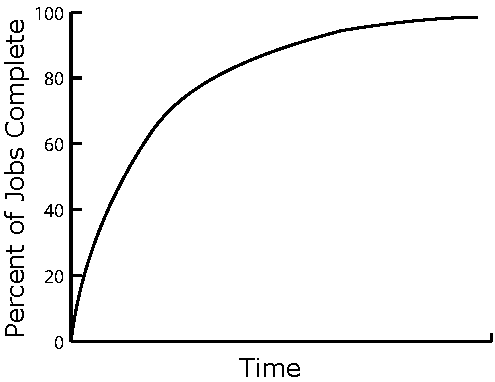
\includegraphics{figure/grid_job_completion}
    \caption{Grid jobs return most results quickly. Later results tend to take much longer to return. Physicists may with to check data before all results have returned.}
    \label{fig:grid-job-completion}
  \end{center}
\end{figure} 
He looks at the existing results by hand, meaning that he logs into a machine that has the results and interactively runs a short analysis against the file. Then he wants to run a SW Framework analysis against what parts of the first analysis are complete. He constructs a new analysis specifying the currently available results as input and submits that job to run.
\end{narrative}

\begin{narrative}{Mark a Block of Runs or Events as Bad}
Even though events passed validation at the detector and reconstruction, it is possible for them to have a problem that precludes using them. It is possible that the reconstruction was good but that an analysis step later had a problem. For instance, there may be a cluster node with a bad FPU. A physicist tells the data manager that there is a problem. Instead of rerunning the analysis, a data manager wants to exclude certain events in such a way that physicists doing analysis will not accidentally get the bad events when they specify this sample. At the same time, the data manager may not yet be prepared to remove those events from the dataset, possibly because having the bad events around could be crucial to understanding imperfections in earlier analysis.
\end{narrative}

\begin{narrative}{Compare Why Two Analyses Had Different Results}
Two scientists are looking for the same type of physics event. Given the same starting base reconstruction, one got sixteen events, and the other got three. They want to find what was different between the two analyses, so they look to see as much as they can about the processing each one did. Which datasets did they use? Which versions of processing did they use along the way? During processing, some subset of the parameters were relevant to the physics of the results. Were those parameters the same, or how were they different? (Elaborate on what parameters to compare.)

One way to compare analyses is to run the three-event analysis on the sixteen events from the other analysis.
\end{narrative}

\begin{narrative}{Publish a Dataset to Global Scope}
Physicist Phil runs his own analysis on RECO data. He makes a new skim and publishes it to the local DBS for his group. His group takes a look at it, and they think it's a great skim for their research and for others. The Data Quality Group meets and says it is wonderful. They create an Analysis Dataset from this skim, throwing out only the first and last lumi blocks, just out of habit because they tend to be worse than most others. Then they publish his skim to the world by putting it into global scope.
\end{narrative}
What tools would they need? Assuming a Data Quality Group analyzes a dataset using ROOT or cmsRun, they can write a list of good lumi blocks, but then something must accept them to the DBS and verify all information is there. Then a tool must request that the DBS publish data from local to global scope.

\begin{narrative}{Recover Failed DBS}
If the DBS machine fails, is there failover to take its place? How do you reload a DBS? If the DBS information for a dataset were completely lost, what kind of information exists to reconstruct its provenance? How could you insert such provenance into the DBS?
\end{narrative}

\begin{narrative}{Troubleshoot Problems with Detector Operation Using Analysis Output}
At Compute Tier 0, tracking efficiency looks like it fell off in the HLT. Maybe output of the prompt reconstruction will be clearer about whether there is a problem or not, so a detector expert wants to look at prompt reconstruction data. The analysis program could be written in SW Framework or in ROOT. Even though the prompt reconstruction has not yet processed all the data that will become the next reconstruction dataset, the detector expert wants access to the data that has been processed. It may be that it is someone's job to check the first events that the prompt reconstruction produces.
\end{narrative}

The detector expert may specify a data range by specifying that they want the reconstruction for a set of events within a run, but they will need some earlier knowledge of which events are being written at a particular time.

\begin{narrative}{Validate Reconstruction Production is Working Well}
A reconstruction expert wants to make sure that the reconstruction is going well, so they check the first few events of the reconstruction at regular time intervals. The reconstruction job is still in process, and there is not yet a complete dataset. The reconstruction expert wants to run a SW Framework or ROOT job against the first events.

If the reconstruction is not working well, this expert has to stop reconstruction, ensure resulting data is not used, and then either restart processing of RAW data or contact the detector expert to troubleshoot. 
\end{narrative}

\subsection{Use Cases for Data Management Applications Interacting With DBS}

\begin{usecase}\label{uc:generalanalysis}
\ucname{Conduct a Physics Analysis} \\
\ucactor{Physicist, Prodagent or CRAB, a DBS} \\
\uclevel{High Level} \\
\ucscope{Application Scope} \\
\ucdescription{This high level use case is a placeholder for the steps involved in submitting a job of any sort, whether a production job or a physicist's analysis job at Tier~5. We will use Prodagent as the name for the job submission tool, but this will be generic.} \\
\ucrevision{Draft} \\
\uctrigger{Physicist has an idea for analysis, including the type of physics events of interest and a conceptual view of which analysis products will be necessary, such as tracks or jet reconstruction.} \\
\ucsuccess{\begin{uclist}
  \item Data Discovery Tool provides best available dataset.
  \item Discovery Tool provides summary information about that dataset, suitable for job submission.
  \item Physicist provides dataset summary information to Prodagent.
  \item Prodagent requests \phedex data, if required.
  \item Prodagent runs the job.
  \item Prodagent provides Physicist with a Local DBS entry containing dataset with correct provenance.
\end{uclist}} \\
\end{usecase}

The actual steps entailed in data discovery are largely a matter of the user interface. We describe data discovery in another section because it can be described more concisely than in use cases.

The first detailed use case is about how Prodagent or CRAB works with the DBS. It tries to cover both the case where the input dataset and output dataset are in the Local DBS or Global DBS. Note the Prodagent-Local DBS is an instance of the DBS which lives just for the sake of Prodagent to construct correct provenance information to give later to the correct receiving DBS.

\begin{usecase}\label{uc:generaljob}
\ucname{Run an Analysis Job} \\
\ucactor{Prodagent, Prodagent-Local DBS, Global DBS} \\
\uclevel{Goal Level} \\
\ucscope{Service Scope} \\
\ucdescription{This describes how a workflow system, such as Prodagent or CRAB, runs a grid job on behalf of a user. It will read configuration files, generate the appropriate input to SW Framework or ROOT, and then run the job wherever it is told.} \\
\ucrevision{Draft} \\
\uctrigger{Physicist provides a configuration file. Foremost in it is the dataset specification which consists of the dataset name, a triple of primary dataset, data tier, and processed dataset or analysis dataset. To this, the physicist may add a further specification of lumi sections for real data or event ranges for MC.} \\
\ucsuccess{\begin{uclist}
\item Prodagent checks Global DBS for input dataset file block ids.
\item DLS tells Prodagent where the LFNs corresponding to those file blocks are located.\label{uc:gen_avail}
\item Global DBS provides dataset LFNs corresponding to requested lumi sections and the list of lumi sections.
\item Prodagent records tracked parameters from configuration files in parameter database.
\item Prodagent creates processed dataset in Prodagent-Local DBS. It provides the input processed or analysis dataset with lumi sections, the application with version and a pointer to the tracked parameters.\label{uc:gen_create_ds}
\item Prodagent constructs files for grid submission.
\item Appropriate Grid manager executes job at requested computing site.
\item As jobs return, Prodagent puts the files into the Prodagent-Local DBS, associating them with the output processed dataset. When there are enough files, it consolidates them into file blocks and registers these with the Prodagent-Local DBS.\label{uc:gen_jobs_return}
\item Prodagent registers completed job in Global DBS or Local DBS, as requested. It gets this information from the Prodagent-Local DBS.
\end{uclist}} \\
\ucextensions{\begin{ucextlist}{\ref{uc:gen_avail}}
  \item Dataset is not available at processing site.
    \begin{enumerate}
    \item \phedex transfers those file blocks, specified by LFN, to the correct site.
    \item Prodagent checks DLS to see when data arrives.
    \end{enumerate}
  \item Dataset is in Local DBS, not the Global DBS.
\end{ucextlist}
\begin{ucextlist}{\ref{uc:gen_create_ds}}
  \item Dataset already exists.
\end{ucextlist}
\begin{ucextlist}{\ref{uc:gen_jobs_return}}
  \item Some jobs fail to return.
  \begin{enumerate}
    \item Prodagent registers all files which have returned.
    \item Prodagent consolidates last files into file blocks when instructed by Physicist to terminate job.
  \end{enumerate}
\end{ucextlist}} \\
\end{usecase}

Who specifies what will be the data tier of the output processed dataset?



Prodagent Accepts Several Datasets as Input to an Analysis with a Single Output Dataset

Prodagent Configures Monte Carlo Generation to Match Given Data Dataset

Provenance Tool Assembles Metadata on the Processing of a Dataset

Provenance Tool Publishes a Dataset to Local Scope


Provenance Tool Compares the Processing of Two Datasets

\phedex Transfers Dataset Files for Tier 2 Production

\phedex Keeps a Dataset Updated with Newly-Produced File Blocks

Workflow Tool Runs Prodagent

Prodagent Runs Tier 0 Production of Monte Carlo and RECO 

\section{Data discovery needs and options}

\subsection{Needs for Data Discovery}

\subsubsection{Data discovery}

 need a clear definition of ``data''
 who are the actors
 versioning
 level of granularity
 push or pull model
 data, meta-data, luminosity ....
 descriptive criteria

\subsubsection{Data discovery prototype}
The current DBS Data Discovery prototype has been shown on Figure \ref{fig:dbs-data-discovery}.
\begin{figure}[hbtp]
  \begin{center}
    \resizebox{10cm}{!}{\includegraphics{figure/DBSDataDiscoveryLayers.eps}}
    \caption{DBS Data Discovery prototype.}
    \label{fig:dbs-data-discovery}
  \end{center}
\end{figure} 
It based on three external third party packages:
\begin{itemize}
\item {\it CherryPy}~\cite{CherryPy} is the a pythonic, object-oriented HTTP framework.
It has been used as a simple web server for DBS data discovery proptotype.
\item {\it Cheetah}~\cite{Cheetah} is the template engine and code generation tool, 
written in Python. It can be used standalone or combined with other tools and frameworks. 

\item {\it SQLAlchemy}~\cite{SQLAlchemy} is the Python SQL toolkit and Object Relational 
Mapper that gives application developers the full power and flexibility of SQL. 
It provides a full suite of well known enterprise-level persistence patterns, 
designed for efficient and high-performing database access, adapted into a simple and 
Pythonic domain language. It works with well-known DBs, including: ORACLE, MySQL, Postgres, SQLite, 
etc.
\end{itemize}

The multi-tier architecture of the server will allow the usage different type of technologies, e.g.
SQLAlchemy can be replaced with generic Database accesing layer, such as JDBC or Database
connection pool management, CherryPy with apache web server, etc.~\cite{frontier}.

We try to explore the way how physicists will discover new data within CMS experiment. First,
we see clear division between our actors. They are:
\begin{itemize}
\item {\bf physicists} -- this category includes people whose interests extend to identify
data avaialable for analysis, e.g. find Higgs sample which pass certain criterias.
\item {\bf production managers} -- this is a list of actors who are mostly interested in
data production and deployment.
\item {\bf site administrators} -- this category of users are interested in monitoring site
resources, such as disk usage.
\item ...
\end{itemize}

In current prototype we mostly address the CSA06 use casses, the {\bf production manager's} 
point of view to discover data. We start from identifying file blocks based on three 
main search categories:
\begin{itemize}
\item application -- identifies details of software used for data production, e.g. 
CMSSW\_0\_8\_1, as well as the production step, {\it family}, e.g. RECO, and 
name of the executable, e.g. cmsRun.
\item primary dataset -- identifies primary dataset, e.g. CSA06-081-os-minbias.;
\item data tier -- identifies data tier, e.g. RECO.
\end{itemize}
The presentation layer, auto-generated using Cheetah~\cite{Cheetah} templates, represents
the {\bf physicists} and {\bf experts} (such as {\bf production managers} output.
Their difference lies in fine-grained details of data, for instance pn {\bf expert} page
the block/file statuses are shown, while {\bf physicists} output hides such detail and shows
only valid samples useful for generic analysis.

The following extensions are quite visible to implement:
\begin{itemize}
\item list of avialable sites together with details of data on those sites, e.g. for site A we 
summarize the total disk usage, location of files, etc.
\item list of run/lumi-sections
\item list of avaialble datasets with full description of them, e.g.
electron -- electron trigger signal
\item list of applications with full description about their configurations, etc., e.g.
CMSSW\_0\_8\_1 version which includes the following list of config files
\item form which will allow to find parentage information about particular dataset
\end{itemize}

The long term plan may includes development of user-freidnly queriable language for 
data discovery.
\subsubsection{Data to discover}

 we need to discover at least the following items:
 files, file blocks, event collections, runs, datasets,
meta data, data types (e.g. MC/reco)
 But actors have different vision for data discovery:
 Production interested in: files, file blocks, event
collections, data type
 Physicists interested in: event collections, datasets,
runs, meta-data, data type
 data managers/site admins: files


\subsubsection{Meta data}

 Which kind of meta data physicists wants:
 run, dataset, trigger stream, energy, ...
 how they want to express their requests
 who is going to generate meta data
 how meta data will be populated to DBS?
 where meta data will be stored

\subsubsection{Actors behavior}
 we need clear understanding how different actors
behave
 Physicist wants to perform manual discovery at initial step
of analysis and automate the process later
 Phedex will/should perform auto discovery
 site admins/data managers will do it periodically and make it
semi-automatic
 we need a set of tools to support such behavior

\subsubsection{Data indexing}
 All actors mostly interested in fast data access
 DB vs file based indexing
 data indexing level: file block, files, evcoll, ...

\subsection{Possible tools for indexing}
We need to be able to provide search capabilities on the data that most interests analysis use-cases. 
The important parts of bits are in Parameter-Sets that describe how datasets/files are produced.

What we have today in DBS is just a place holder and no real use.
We need to define how we want to store Parameters-Sets in DBS and keep in mind that they are easily search-able.
We can individually add and describe parameter-set(s) into DBS (for example).
This is Pre-requisite to search and discovery, if we don't have parameters-sets organized somewhere we can��t index/search them too.

Many interesting ideas/tools exists out in the wild, we need to define the Requirements. 
I say we need to index the parameter-sets and some other characteristics of datasets to make them search-able. We might need to create some definitions and mappings too.
Names that comes to mind a Google, LXR, Apache Lucene.
We need something that doesn��t return 10,000 pages (google type searches are out), that, specific to our needs could be tailored (Lucene is in), be capable of searching for specific keywords that makes sense to users but are not actually in the files (LXR is out!). [Sort of maps between what files hold and what it means].


http://lucene.apache.org/java/docs/index.html
Lucene is Doug Cutting's wife's middle name, and her maternal grandmother's first name !. 
Apache Lucene is a high-performance, full-featured text search engine library written entirely in Java. It is a technology suitable for nearly any application that requires full-text search, especially cross-platform. 
open source project.  
Lucene is 100% pure Java and has no external dependencies. 
Provides search and indexing capability, one can write his/her own indexing mechanism and rest is taken care off.
This is shown in  Fig.~\ref{fig:dbs-indexing} and described in this section.
\begin{figure}[hbtp]
  \begin{center}
    \resizebox{15cm}{!}{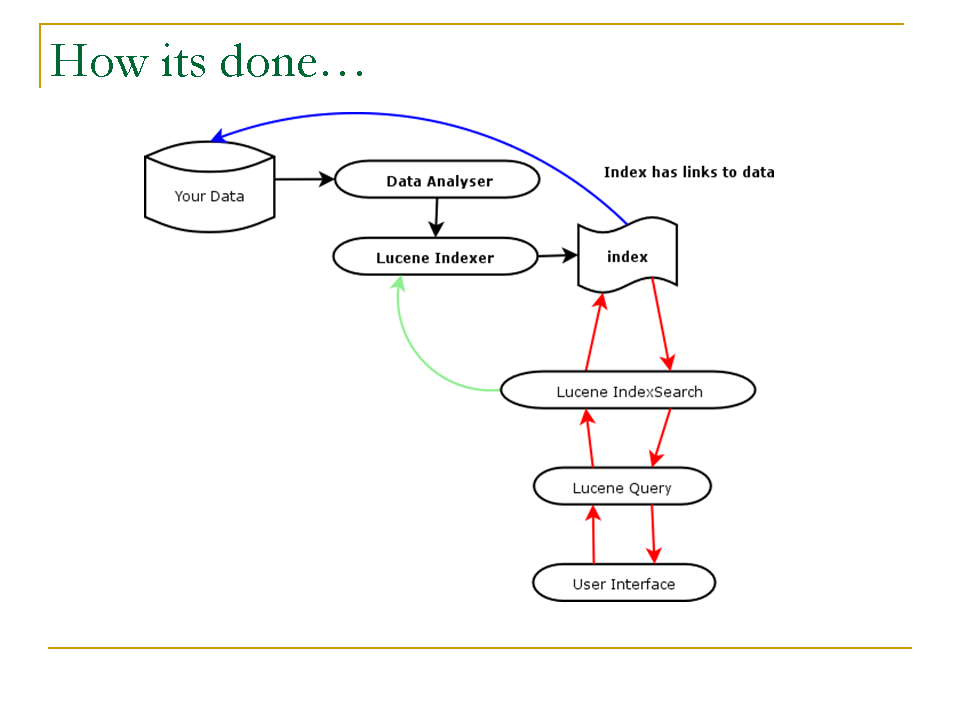
\includegraphics{figure/DBS_Indexing.eps}}
    \caption{Using a tool, such as Apache Lucene, to index parameter files.}
    \label{fig:dbs-indexing}
  \end{center}
\end{figure} 

Indexing Characteristics
\begin{enumerate}
\item over 20MB/minute on Pentium M 1.5GHz
\item small RAM requirements -- only 1MB heap 
\item incremental indexing as fast as batch indexing 
\item index size roughly 20-30% the size of text indexed 
\end{enumerate}

Searching Characteristics
\begin{enumerate}
\item ranked searching -- best results returned first 
\item many powerful query types: phrase queries, wildcard queries, proximity queries, range queries and more 
\item fielded searching (e.g., title, author, contents) 
\item date-range searching 
\item sorting by any field 
\item multiple-index searching with merged results 
\item allows simultaneous update and searching 
\end{enumerate}





\section{Framework needs}


This is shown in  Fig.~\ref{fig:framework-access} and described in this section.
\begin{figure}[hbtp]
  \begin{center}
    \resizebox{15cm}{!}{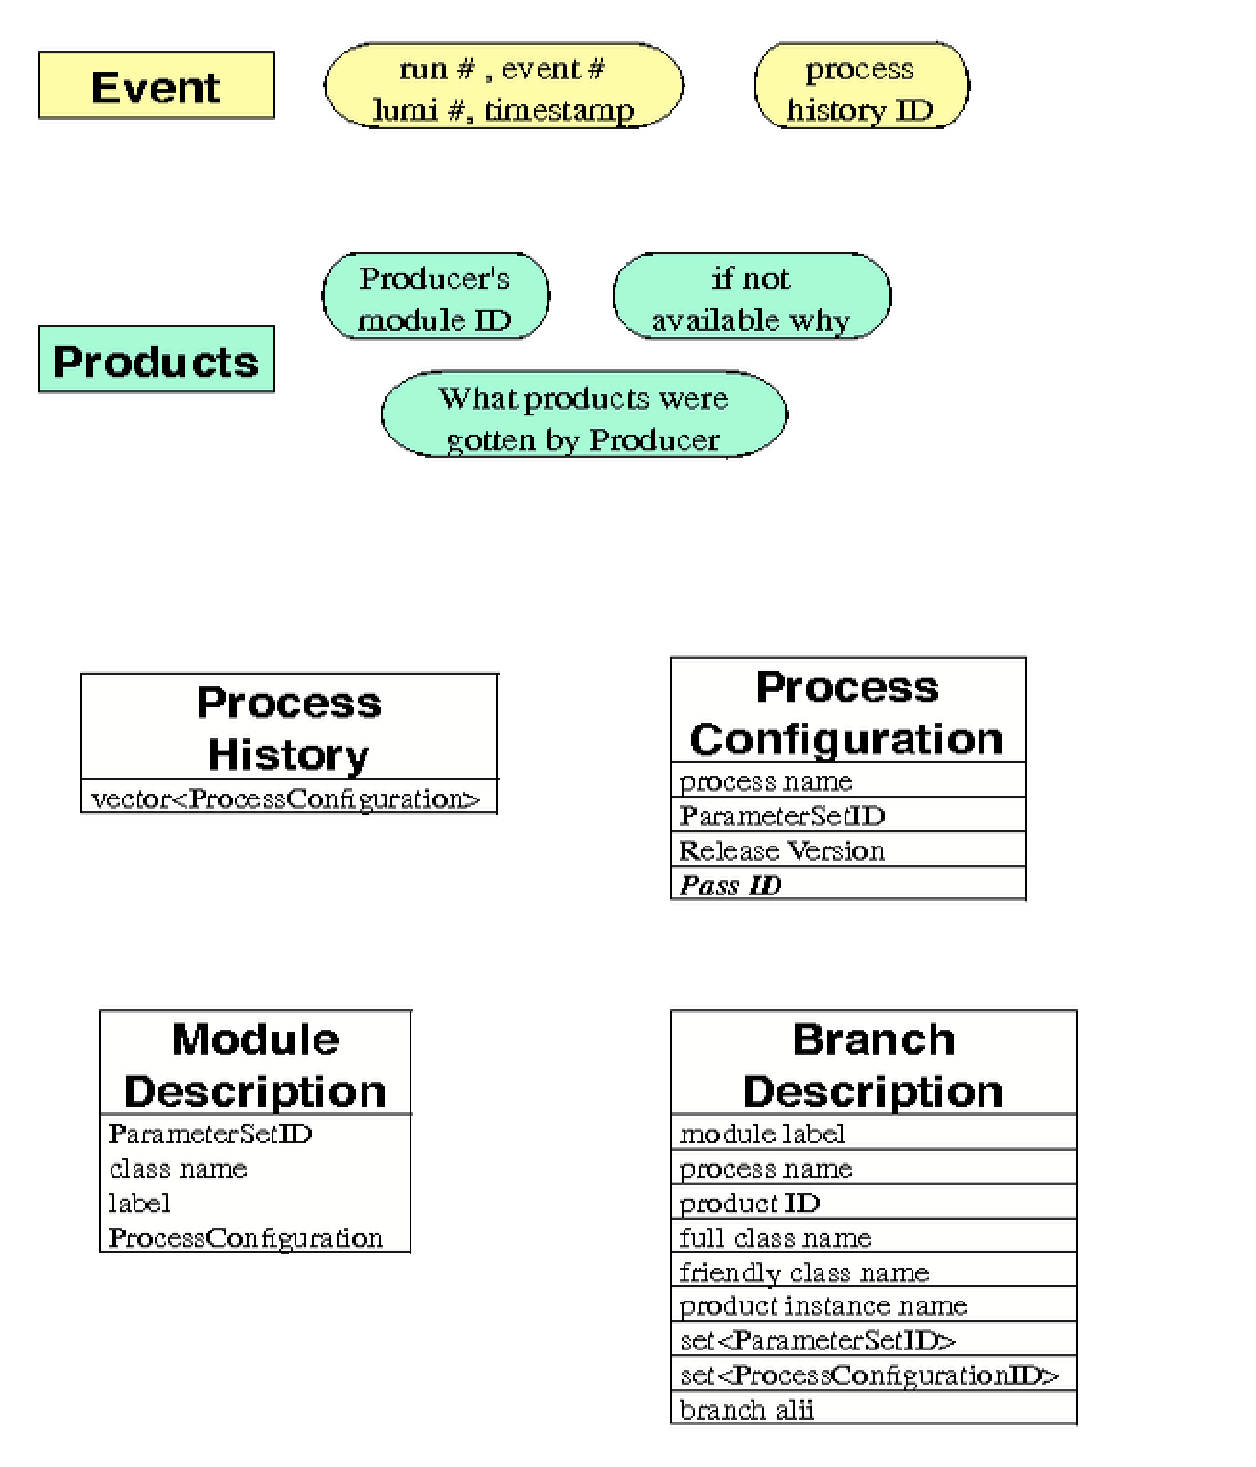
\includegraphics{figure/access.eps}}
    \caption{CMSSW Framework access.}
    \label{fig:framework-access}
  \end{center}
\end{figure} 

\subsection{CMSSW Framework provenance/DBS interaction}

The "Unambiguous identification of reconstruction results" section of the "CMS Core Software Re-engineering Roadmap" is mostly correct (a few things are not implemented yet, and some recent design decisions are not reflected there yet). This page provides a brief summary of the the aspects of the framework provenance which may have implications for the DBS provenance database.

\subsubsection{Framework provenance summary}

There are two kinds of provenance produced by the framework: (1) module configuration for the process; (2) event-by-event, for each object produced, what event objects were accessed by the module producing that object. Event-by-event provenance is dropped if the objects are dropped (TODO: verify); module configuration is always stored (it was decided that garbage-collecting unreferenced configurations was not worth the effort) (TODO: verify). Dropping the event-by-event provenance can lose processing history, since only direct parentage is kept (TODO; verify), but the sequence of processing steps is stored. The module configuration stored is currently the configuration for the entire process (i.e. the union of all the module configurations) (TODO: verify), not a module-by-module configuration, but the module by module configuration can be recovered from the overall process configuration. Provenance tracking for the EventSetup is planned, but not (as of May 2006) implemented yet. The full provenance is written to the output file.

Names/paths of files containing event data are untracked parameters, so they are not recorded in the provenance. There are also no file unique identifiers--the framework, except for the input and output modules, deals with events as objects with no association with any file. Filenames of some conditions data are tracked parameters.

Each CMSSW production process has a "job configuration" name. The job configuration name is a component of the branch name for objects produced in that job, so branch names will be different for objects where the processing steps differ (e.g., SIM/DIGI/RECO in one job vs. three separate jobs). The framework partially hides this, but it is visible in ROOT, so there is a strong incentive to use an identical sequence of processing steps for all objects of a given type. As of May 2006, there are proposals for aliasing branch names which may change this consideration if every branch has an explicitly configured alias.

EDM fast merge will, in one job, only process files with identical provenance. Prior to the 0.8.0 release, the CMSSW Framework had the same restriction. Starting with 0.8.0, CMSSW plans to support "fruit salad" processing, where files with different provenance may be processed in the same job if the provenances are compatible. Provenances are considered compatible if the object name to number mappings are the same for all objects in common between the files. The fast merge does not modify any objects, and does not create any provenance--so far as CMSSW is concerned, fastmerge is completely transparent.

\subsubsection{DBS implications}

At the file level of the DBS, the CMSSW provenance mostly provides constraints. File parentage must be tracked entirely by the DBS--CMSSW does not track it. CMSSW provenance provides a processing history at the object level, not the file level, and the object history may not be a complete record of the processing steps that produced the file containing that object if intermediate objects have been dropped from the output.

The framework allows objects of the same type but different provenance if they differ in the process name, process instance label, or module label. The framework provenance may also include module configurations for objects which are not in the output file, since module configurations are not "garbage collected". The presence of multiple configurations for the same module--for objects which may not even be in the corresponding files--will limit the accuracy and reliability of queries on any "file level" provenance summary. A simple example of this would be if the HLT places reconstructed objects in the output stream which are also produced in prompt RECO or re-reconstruction. At the very least, this would mean that any query on the DBS provenance must include the process name as part of the query, and that may not be sufficient for the analysis use cases envisioned.

\subsubsection{Notes and links}

    * How to Configure Output Modules documents how branch names are constructed
    * EDM Paths and Trigger Bits explains how to selectively write events based on "trigger" paths
    * The framework currently reads only one data file at a time--there is no ability to join data from multiple files in the baseline. Adding this ability is (as of June 2006) under discussion. 

\section{Schema Description and Design}

During the Workshop we started a design for a new schema to supered the one being used for CSA06. This has been drawn and several modifications added to reflect the entire Workshop discussion and decisions made there. This is shown in  Fig.~\ref{fig:new-dbs-schema-design} and described in this section.
\begin{figure}[hbtp]
  \begin{center}
    \resizebox{15cm}{!}{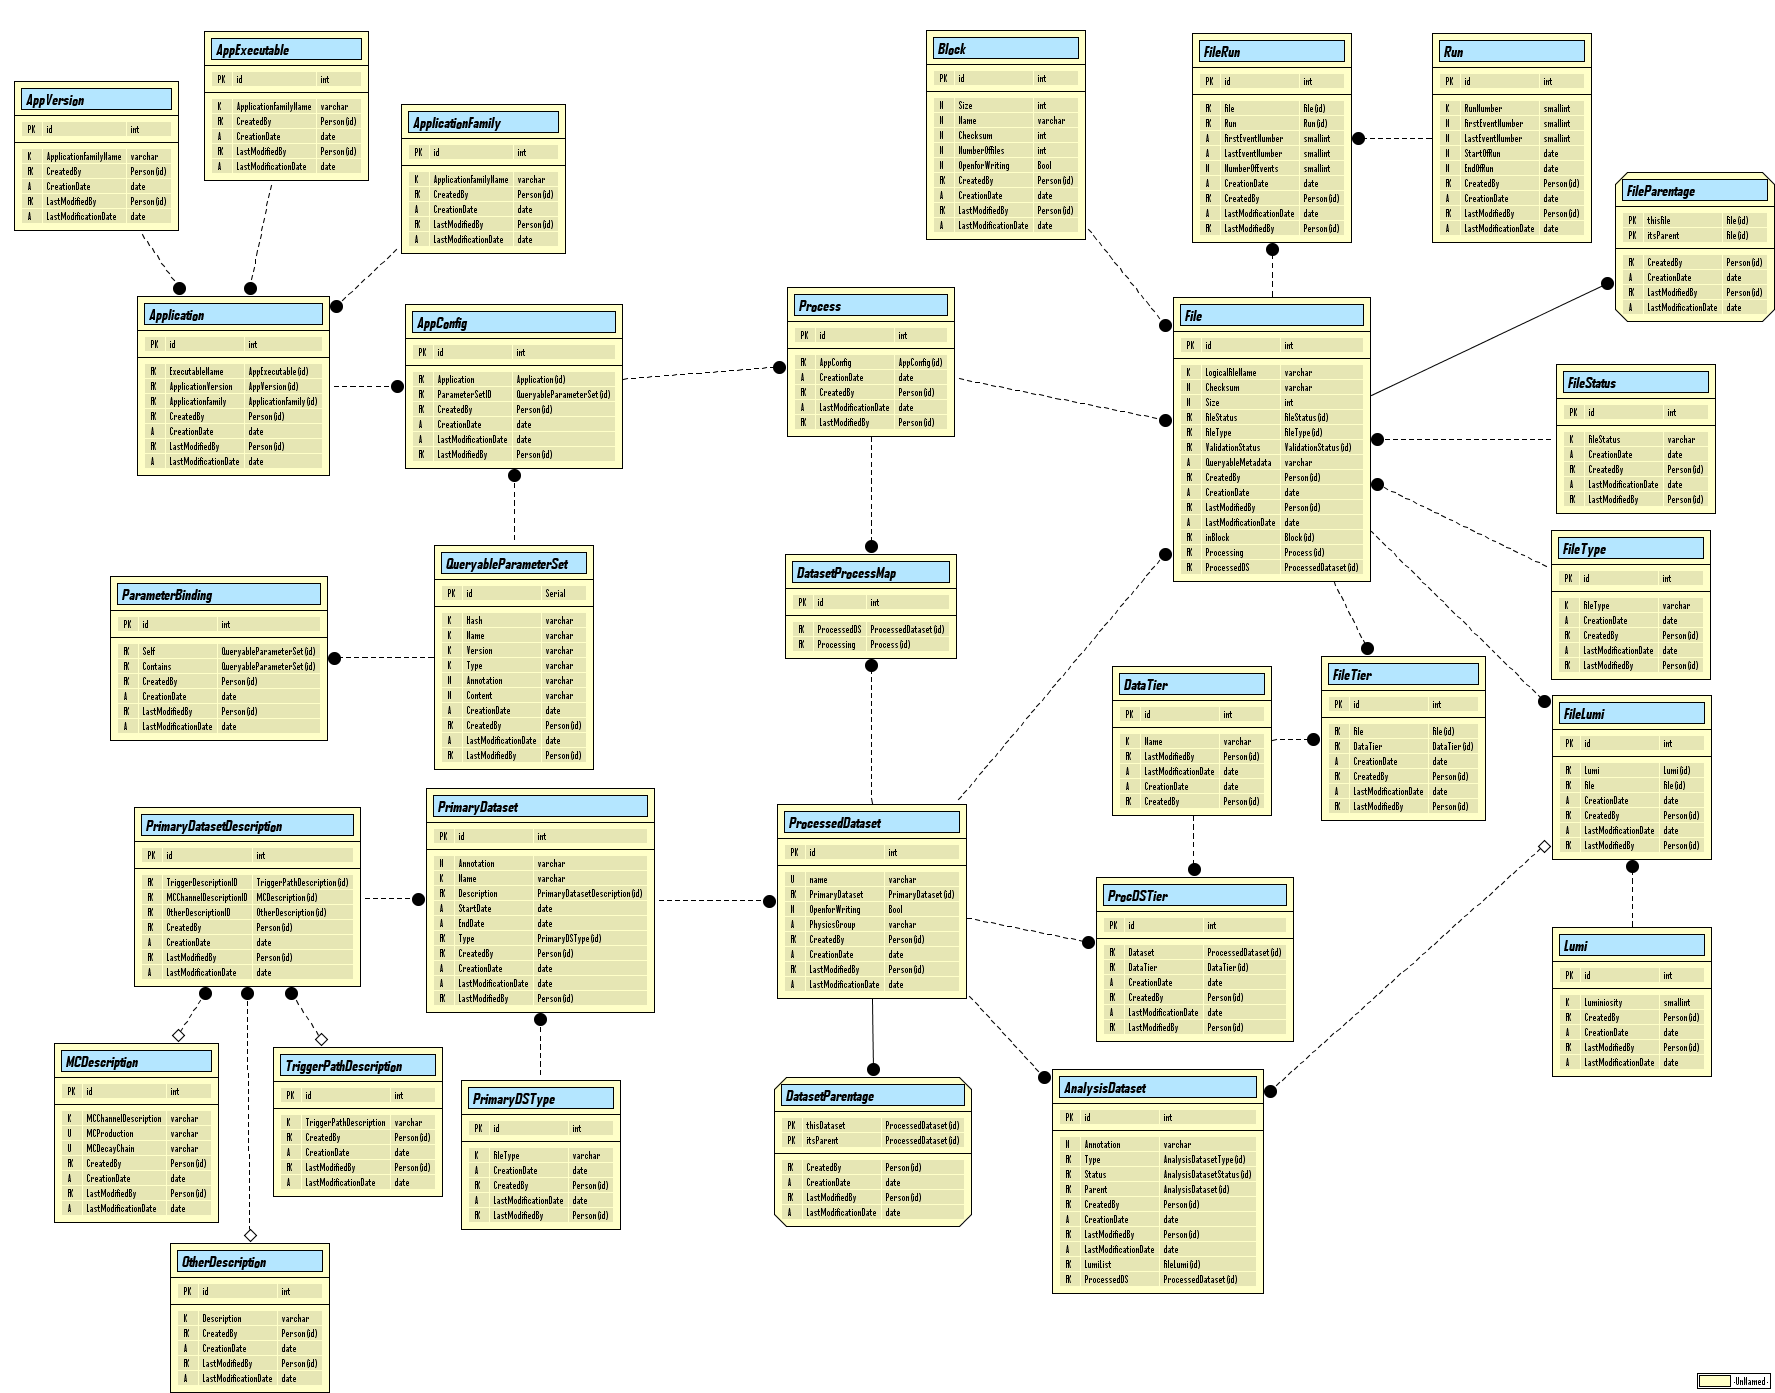
\includegraphics{figure/schema_07272006.eps}}
    \caption{New DBS schema design.}
    \label{fig:new-dbs-schema-design}
  \end{center}
\end{figure} 


\begin{enumerate}
\item{File}
 A File can contain multiple runs. A run can contain multiple files. The
 event range in a file represents the lowest bound event number to the
 highest bound event number. For example in a run r with a File f has
 event range 19,130. This does not imply that all the events are
 contiguous . There might be some events that can be missing. For example
 in this file f , only events 19,20,25,130 are present and rest of then
 are bad or missing.
 
 \item{FileRun}
 This table will represent many to many relationship in file and run.
 Note that the event range is an attribute of the FileRun table and not
 just of the File Table. This is required when multiple files will be
 merged into one single file. Then a File can spawn multiple runs and can
 spawn multiple event ranges. To discover all the event in this file we
 need to make event range an attribute of FileRun table. For example say
 a file f1 in run r1 contains events 3,16 and file f2 in run r2 contains
 events 5,15 and file f3 in run r1 contains events 2,13 . After we
 can merge f1,f2 and f3 into a big file ff, now FileRun table would
 contain two entries for file ff and run r1 and run r2. First entry for
 ff,r1 would have event range 2,16 and another entry for ff,r2 would
 contain 5,15. Note that of the files to be merged are in the same run
 then the event range would be minimum of lower bounds to maximum of
 higher bounds min(3,2),max(16,13).
 
 \item{FileParentage}
 This represents the lineage of the file. All the parents of the file are
 represented in this table. This file parentage is required at the file
 granularity. If it is not presents at this granularity , then there
 would be no way to correctly determining the exact parent of any
 particular file. Please note that this parentage is also specified at
 the ProcessedDataset level. The only reason for that is the optimization
 for discovery. One can easily find the parents of a dataset via
 traversing all the files and finding the parents of those files and then
 locating the datasets those files exists in. To optimize this discovery
 we need parentage at the dataset level too.
 
\item{ Block}
 This entity is entirely a concept of size and number of files. It can
 contain many files but if the collective size of those files reaches a
 certain limit (can be set by DBS admins), then it cannot accommodate any
 more files in it. In that case a block can be closed and a new block can
 be opened for adding new files into it. A block can be uniquely
 determined by its name that can also include dataset path along with its
 id.

(Dan's comments)
As was pointed out to me at the workshop, a block is supposed to
be homogeneous--all the contents should of a block should be of
the same data tier and processed data set.  This is important for
PhEDEx and for some of the management data discovery use cases we
discussed at last Friday's meeting.  PhEDEx in particular needs to
be able to efficiently find all the blocks for a given data tier
and processed data set, so this constraint may need to appear in
the schema as an optimization.
 
 \item{Lumi}
 A file can contains many Lumi Sections and a Lumi Sections can be
 contained in many files. These Lumi Sections are used for describing an
 analysis dataset which is conceptually more or less not related with
 files.

(Dan's comments) Missing here is what a luminosity section is.  The definition can be
found on this page:

https://twiki.cern.ch/twiki/bin/view/CMS/CMSTORTagonline

What's relevant for the DBS is that a luminosity section maps
onto a (contiguous) set of events defined at the time the data
are taken.  Since the the luminosity section boundaries are
defined by the DAQ, they will never change.  Luminosity sections
are not supposed to cross file boundaries--when the framework
splits a file for size limit reasons, it is supposed to do so
at a luminosity section boundary (I don't believe this is
implemented yet).

\item{DataTier}
 DataTier is infact related with the AppConfig via ParameterSet. But we
 need DataTier linked with Files also , since a physicists would require
 to know all the file in a dataset which has a certain DataTier. If
 DataTier would just be an ProcessedDataset Attribute, then the above
 query could not be executed. This is because a ProcessedDataset can
 spawn multiple DataTiers. If there is a restriction that a
 ProcessedDataset would only have a single DataTier then we would not
 required DataTier linkage with files at all. Also a File can have
 multiple DataTiers also, that is why all the more reasons to link
 DataTier with File. Note that FileTier is enough for associating and
 determining the DataTier with in a file as well as within a
 ProcessedDataset. So why would we need linkage of DataTier with a
 ProcessedDataset. The reason is same as that of File Parentage and
 ProcessedDataset Parentage. This is just an optimization for determining
 the DataTier with in a DataSet. One has to traverse all the files
 otherwise to know the DataTiers.

(Dan's comments)

As you note, a single AppConfig can write multiple files of different
data tiers at the same time, so the AppConfig <-> data tier
relationship is ambiguous.  The new definition of data tier is that a
data tier comprises a list of objects defined by a release which are
written to files of that tier.  The objects written to a file of a
given data tier will be defined by a release-dependent configuration
fragment, so what objects go into an AOD or RECO file may vary from
release to release.  I don't know how practical it will be to retrieve
these lists from the full ParameterSet -- it may be desirable to have
a separate table mapping (data tier, release) to a list of objects.
 
 \item{PrimaryDataset}
 PrimaryDataset is a placeholder for any type of data like raw or
 production. It is determined by the name and the description. Now this
 description can be of 3 different types: Monte Carlo type, Trigger Path
 type or some Generic Description. Therefore there are 3 tables
 representing each one. PrimaryDataset can contains raw data which means
 that it was not processed. To manage this within the schema, one can
 create a dummy ProcessedDataset with no link to any Application
 (AppConfig in this case). All the raw files can now be placed in this
 dummy ProcessedDataset

(Dan's comments)

There's actually two kinds of raw data: DAQ-RAW is the raw response
data from the detector in FED format, which is input to the HLT; RAW
is the output of the HLT.  Normally what will be injected into the DBS
is RAW data from the HLT, and the HLT is a cmsRun application with a
standard parameter set, so the normal RAW data will have real
processed data sets, not a dummy one.

 
 \item{Application}
 Application is uniquely determined by the Application Version,
 Application Executable and Application Family. There are three table
 representing each one and collectively they represents an Application
 \item{ParameterSet}
 ParameterSet is a collection of Parameters which are used to make a
 process. An entry in the ParameterSet can represent a single parameter
 or a composite parameter. For example a single parameter would contain
 name, value ,type and hash and a composite parameter would contain
 name, value ,type and hash  with or without content. Also a composite
 parameter would contain lot of other single or composite parameters.
 This is represented by the ParameterBinding table. One can look at these
 as a hierarchical directory structure. A single parameter would be
 lowest level directory which does not contain any other directory. A
 composite parameter would be a directory that may or may not contain
 other directory and may or may not contain a file (content). Hash
 uniquely identifies a parameter (both single and composite)
 
(Dan's comments)

I believe there's a way of getting the framework's pset parser to
give access to its internal parse tree, which could be used to
construct the QueryableParameterSet.  Parameter set's can have
fairly complicated nesting, so I'm a little worried about what a
query on this will look like, but I guess this is a reasonable
starting point.

 \item{AppConfig}
 A unique combination of an Application and a ParameterSet would
 represent an AppConfig. A file will be produced by a single AppConfig.
 That is why we have many to one relationship between AppConfig and File
 table. Note that a File has a relationship with ProcessedDataset, but
 that is not enough to determine the exact AppConfig used to produce the
 file. The reason being that a ProcessedDataset can spawn multiple
 AppConfig.
 
(Dan's comments)

While this is true, keep in mind that the framework can now merge
files with different provenance (the "fruit salad" mode), so different
objects in a single file may have different parentage/processing
history.

\item{ ProcessedDataset}
 Is uniquely represented by the PrimaryDataset , AppConfig and the input
 ProcessedDataset if any. Also, a ProcessedDataset can contain various
 AppConfig (Different version of Application). This satusfy the use case
 of creating many files with same application but different version of
 the software used. It can contain multiple files and therefore has
 one to may relationship with file. Also it can contain multiple DataTier
 which itself can spawn multiple ProcessedDataset and therefore many to
 many relationship among them. The reason for this linkage is for
 optimization purposes only and is described in FileTier section
 
 \item{AnalysisDataset}
 It is uniquely determined by Lumi Sections and ProcessedDataset. An
 AnalysisDataset is a subset of ProcessedDataset. From one
 ProcessedDataset many AnalysisDataset can be derived. Driving a new
 AnalysisDataset from an existing AnalysisDataset would mean to create a
 new ProcessedDataset. So essentially it will be a new AnalysisDataset
 from a ProcessedDataset again. Also AnalysisDataset can contain many
 Lumi Sections and same Lumi Sections can spawn multiple AnalysisDataset.
 Therefore we have AnalysisDSLumi table which represents many to many
 relationship among these entities.

(Dan's comments)

Analysis data set is more complicated than this.  The definition we've
been using is "a list of luminosity sections which were specified by
running an analysis query on a processed dataset at a particular
instant of time".  A processed data set may contain multiple instances
of a luminosity section processed with different application
configurations, so an analysis data set is determined by a processed
data set, a list of luminosity sections, and an AppConfig for each
luminosity section.

We haven't discussed how (or if) this maps onto MC data.
\end{enumerate}
\section{Client API}
\subsection{CSA06}
Python based (2.4.x and backward).
No external dependencies.
Independent of server implementation.
Exchange Python objects and Python data types with client(s).
Defines Client Data Structures/Types (CDS) for convenience (Derived from Python dictionary). CDS implement strict type checking for good reasons.
Throws DbsApiException.
Currently covers CRAB and Prod. Use-cases. Analysis use-cases are targeted during DM/DBS workshop at Cornell in July. 
Some dataset discovery APIs are also present, though we are in stone-age of dataset discovery. 
http://cmsdoc.cern.ch/~sekhri/Html/mc.htm
API Documentation at,

https://uimon.cern.ch/twiki/bin/view/CMS/CMS-DMS-DBS-API

Currently two type of interactions with DBS,Tpdate and manipulate. 
Update DBS: The key is to understand the insert work flow for each type of information you need to record in DBS. Always a set of API calls in right order will work.
You need to know quite well what you want to do with DBS. Some advanced operatio
ns (Merge/Import/Export) need in-depth knowledge of DBS-API, DBS-Workflow and Da
taset organization in DBS.
FWRK and DBS do not map 1-1 when it comes to Dataset organization. (not here!).
Example: you cannot insert a File Block, before you have inserted Primary Datase
t and Processing.
DBS API is low level API, and calls for an interface layer between client Applic
ation(s), like ProdAgent, and DBS for a real work. One example is ProdAgent DBSI
nterface,
https://uimon.cern.ch/twiki/bin/view/CMS/ProdAgentDBSInterface

Simple use cases are coded in DBS Test cases (part of DBS API code).
Query DBS: Straight forward, you only need to understand ��CDS��, and how they relate to each other. Exposed via above mentioned web-tool.

\subsubsection{The API Structures (Python Implementation)}

Following describes the way dbsAPI Client data types look like schematically.
\begin{verbatim}
DbsPrimaryDataset:
      datasetName (name of primary dataset)

DbsApplication:
      executable 
      version
      family

DbsParameterSet:
      hash
      content

DbsApplicationConfig:
      application
      parameterSet

DbsProcessing:
      parent
      primaryDataset
      processingName
      applicationConfig
      isOpen

DbsProcessedDataset:
      primaryDataset
      processing
      datasetName
      dataTier
      datasetPath
      isDatasetOpen

DbsParent:
      parent
      type

DbsBlock:
      blockName
      processing
      blockStatusName
      numberOfBytes
      numberOfFiles
      fileList
      eventCollectionList

DbsFile:
      logicalFileName
      guid
      checkSum
      fileType
      fileStatus
      fileSize
      block

DbsEventCollection:
      collectionName
      numberOfEvents
      collectionStatus
      datasetPathName
      parentageList
      fileList


Python representation of Client Data Types

We have been working on coming up with a generic dictionary type representation for these types.

For example, a client data type can look like below,

class DbsBase(dict):
     """ Base Class for all DBS Client Data Types """
     def __init__(self, **args):
           dict.__init__(self)


class  DbsProcessedDataset(DbsBase):
   """ 
   Class for ProcessedDataset
   """
   def __init__(self, **args):
      DbsBase.__init__(self)
      self.setDefault("primaryDataset", None)
      self.setDefault("processing", None)
      self.setDefault("datasetName", None)
      self.setDefault("dataTier", None)
      self.setDefault("datasetPath", None)
      self.setDefault("isDatasetOpen", None)
      self.update(args)

class  DbsFile(DbsBase):
   """ 
   Class for File
   """
   def __init__(self, **args):
      DbsBase.__init__(self)
      self.setDefault("logicalFileName", None)
      self.setDefault("guid", None)
      self.setDefault("checkSum", None)
      self.setDefault("fileType", None)
      self.setDefault("fileStatus", None)
      self.setDefault("fileSize", None)
      self.setDefault("block", None)
      self.update(args)

\end{verbatim}

\subsubsection{The API Calls (Python implementation)}
The API will allow the argument for datasetPath to be a string, 
or polymorphicly an object. The string is convenient for users 
entering arguments by hand say, but the object is more convenient when 
using the result returned from another call.   
\begin{verbatim}
[] listDatasets(self, pattern="*"):
\end{verbatim}
   Given a string pattern, provide a list of DbsProcessedDataset objects by name.  The pattern option does not need to have 
three *'s (like */*/*). Returns always a list. If there are none, the 
return will be an empty list.

\begin{verbatim}
[] getDatasetContents(self, (string/obj) datasetPathName)
\end{verbatim}
   (This call is still being discussed with the CRAB developers.) Given a datasetPathName object, or string, return a list of file blocks and event collections. The search proceeds  via the tables processed\_datasets $\Rightarrow$ event\_collection $\Rightarrow$ file $\Rightarrow$ block. 

%************ This call is open for discussion ************
\begin{verbatim}
[] getDatasetBlockContents(self, (string/obj) datasetPathName, (obj) block):
\end{verbatim}
  (This call is still being discussed with the  CRAB developers.) Given a datasetPathName object, or string, and a block object name, returns all files and all parentage information. 
%***********************************************
\begin{verbatim}
?? getDatasetProvenance(self, (string/obj) datasetPathName, dataTierList=[]):
\end{verbatim}
(This call is still being discussed with the  CRAB developers. We need to understand how the provenance is described.)
\begin{verbatim}
   primaryDataset createPrimaryDataset(self, (obj) primaryDataset):
\end{verbatim}
Create a primary dataset and return the same primary dataset back. If
passed an object with the ID already set it will ignore it. 
The authorative source of the PrimaryDataset object ID is always the database.

\begin{verbatim}
   processing createProcessing(self, (obj) processing):
\end{verbatim}
Create a processing and return the same processing back. If
passed an object with the ID already set it will ignore it. 
The authorative source of the object ID is always the database.
\begin{verbatim}
   processedDataset createProcessedDataset(self, (obj) processedDataset): 
\end{verbatim}
Create a processed dataset and return the same processed dataset back. If
passed an object with the ID already set it will ignore it. 
The authoritative source of the object ID is always the database.
What is the significance of "name" for the processed dataset.

\begin{verbatim}
def createFileBlock(self, (obj) block): Refer to processing.
\end{verbatim}
\begin{verbatim}
   processedDataset createProcessedDataset(self, (obj) processedDataset):
\end{verbatim}
   Create a processed dataset with 0 size and 0 files in the block.
\begin{verbatim}
def insertFiles(self, block (defined by processing), fileList):
\end{verbatim}   
Insert the file or files in fileList into the specified block. The number of Files and total size for the block is adjusted accordingly. The table t\_block is locked  when files are being inserted.
\begin{verbatim}
def insertEventCollections(self, (string/obj) datasetPathName, eventCollectionList):
\end{verbatim}
   Remove the rule that EvColls must have Files.
   Remove the other rules about EvColl.
   So each EvColl has a list of "Parent" of object
   With a "type" like PU/Digi etc. Type of parent.
   Parent points to an EvColl.
   Parent EvColl points to parent dataset for parent evcoll.
   EvColl has list of LFN and they go into evcoll\_file table.
   Array inserts, 03 database inserts.
   Go one level parentage.
   Parents MUST already exist.
\begin{verbatim}
  block (list of files) getDatasetFileBlocks(self, (string/obj) datasetPathName):      
\end{verbatim}
Get a list of file blocks. Proceed  via processing $\Rightarrow$ block $\Rightarrow$ files. This call returns empty blocks as well if there are no files in them. This is something PheDEX will need to know. When a file is given to PheDEX 
it needs to know what block it belongs to. 
\begin{verbatim}
[] listPrimaryDatasets(self, (string) pattern="*"):
\end{verbatim}
\begin{verbatim}
[] listProcessedDatasets(self, (string) pattern="*"):
\end{verbatim}
\begin{verbatim}
[] listParameterSets(self, (string) pattern="*"):
\end{verbatim}   parameterSet contents matching, part of contents.
\begin{verbatim}
[] listApplications(self, (string) pattern="*"):
\end{verbatim}
\begin{verbatim}
  pattern= /family/executable/version
\end{verbatim}
\begin{verbatim}
[] listApplicationConfigs(self, (string) pattern="*"):
\end{verbatim}
   pattern=applicationName
>
Consider the usecase of trying to narrow down from a primary dataset,
to a particular tier, to an analysis dataset.  We are missing the 
ability to list dataset tiers, need the call 
\begin{verbatim}
[] listDatasetTiers(self, (string) pattern="*")
\end{verbatim}
The argument could be like /primaryDataset/DataTier, or just DataTier
\begin{verbatim}
[] listFileBlocks(self, datasetPathName):
\end{verbatim}

\begin{verbatim}
def closeFileBlock(self, block):
\end{verbatim}
The block must have an object.
(?BlockName: Processing\#BlockID)




\subsection{Extensions and Changes for next generation DBS}

\section{DBS client server Architecture}
\subsection{Requirements}

+ DBS Access What are the avenues through which the DBS information will be accessed?

\subsubsection{Overview of usage}

   1. Production processing
         1. ProdAgent 
   2. Group processing
   3. Individual processing
   4. Individual and group analysis
         1. CMSSW
         2. ROOT
         3. Other tools, shells, et cetera 
   5. Interactions and relationships with other CMS databases
         1. Trigger, Luminosity
         2. Online Runs
         3. Conditions, et cetera. 

\subsubsection{Access}

   1. API
         1. CRAB
         2. ProdAgent
         3. Framework (CMSSW) through some wrappers?
         4. ROOT ?
         5. Primary language is expected to be Python, but could include C++, Java, et cetera. 
   2. Command Line Input
         1. Designed to work conveniently with standard Unix commands
         2. based on API 
   3. Web tools
         1. Initial tools will use API
         2. May grow beyond API
         3. Include high level search and discovery features 

\subsection{Options for service architecture technology approaches}
There are at least two issues here, 1. server technology, and 2. transport and messaging layer. The two can be closely related as the tools provided for the messaging layer are better for some server solutions than others.
Server options

\begin{enumerate}
\item  CGI/Perl: Continue to develop CGI w/ Perl scripts
\item  CGI/Python: Continue to use CGI, but rewrite scripts in Python
\item  Servlets: Use Tomcat servlet container and implement API in Java servelets.
\item  Commercial Appserver: Use a commercial application server solution, for example JBOSS and Hibernate.
\item  C++ DBS AppSrv?: Reuse the DBS App server developed at FNAL under a standard server technology, like Apache, or Tomcat.
\item  RAD or Agile Web technology: Use one of the recent rapid web development platforms, for example Ruby On Rails (Ruby), or Django (Python), Zope 3. 
\end{enumerate}
Transport and messaging layer
\begin{enumerate}
 \item  Assume the transport layer is HTTP
 \item  Messaging layer can have a couple of choices
         1. Standard like SOAP, XML-RPC, REST
         2. We make something that is performant (like the XML messages used now for CGI, or something similar to Frontier). 
\end{enumerate}
\subsubsection{Criteria for decision}
\begin{enumerate}
 \item  Must be proven technology
 \item  Not out dated
 \item  Well supported by existing tools and documentation
 \item  Flexible framework that we can grow to meet future needs
 \item  Provide needed scalability
 \item  Easily maintainable
 \item  Accommodate schema evolution
 \item  Accommodate API evolution
 \item  Server functions must be well factor-able
 \item  Provide "local" and "global" scope functionality. This implies a. using multiple database technologies and a. having access through local library or remote server.
 \item  Meet performance needs. This depends on transport and messaging layer employed.
\item   Web Services support. This is a desirable, and determines the flexibility for the future. 
\end{enumerate}



The information summary of the areas mentioned above is included in the decision matrix in Table~\ref{tab:tech-options}. Of course this is not completely objective but based on our evaluations and experience we feel that either Tomcat with Java servelets or JBOSS woth Hibernate would be most attractive for long-term development. Of these two we feel that straight Tomcat is quite adequate for our needs and the added features of JBOSS are somewhat overkill for our application. The plan is to use something similar to the existing prototype for the client interface and  xml format for the responses.  Vijay has done some initial testing to verify that the performance is comparable to that measured for the current Perl/CGI prototype. 
\begin{table}[htb]
    \caption{Features provided by each technology option. X=Yes,*=Maybe, but involves more work, ?=Unknown, or too soon to tell, Blank=No  }
    \label{tab:tech-options}
    \begin{center}
      \begin{tabular}{|l|c|c|c|c|c|c|} \hline 
Criteria/Approach & CGI/Perl & CGI/Python & Tomcat w/ Java & Jboss w/&C++ App  &Ruby\\
                  & (CSA06)  &            & Servlets      &Hibernate & Server& on Rails \\ \hline
 Proven           & X & X & X & X & &      \\
 Modern           &   &   & X & X & &    X  \\
 Supported        & X & X & X & X & &    ?  \\
 Flexible         &   &   & X & X & &   ? \\
 Scalable         & X & X & X & X & & ?    \\
 Maintainable     & * & X & X & X & &   ?  \\
 Schema evolution & * & * & X & X & X &   ?  \\
 API evolution    & * & * & X & X & X &  ?  \\
 Easily factorized& * & * & X & X & X &  ?  \\
 Mult DB backends &   &   & X & X & X &   ?  \\
 Accessed via lib 
     or server    & X & X & X & X & X &   ? \\
 Performance      & X & ? & X & X &   &*       \\
 WS Support       &   &   & X & X & * & ?       \\ \hline
      \end{tabular}
    \end{center}
  \end{table}  
%put into tablualr format
%\begin{verbatim}
%Criteria\Approach 	CGI/Perl 	CGI/Python 	Java Servlets/tomcat 	JBOSS/Hibernate 	C++ DBS AppSrv? 	RUBY on Rails
%1. Proven technology 	X 	X 	X 	X 	  	 
%2. Not out dated 	  	  	X 	X 	  	X
%3. Well supported 	X 	X 	X 	X 	  	?
%4. Flexible framework 	  	  	X 	X 	  	?
%5. Scalability 	X 	X 	X 	X 	X 	?
%6. Maintainable 	* 	X 	X 	X 	  	?
%7. Schema evolution 	* 	* 	X 	X 	X 	?
%8. API evolution 	* 	* 	X 	X 	X 	?
%9. Well factorized 	* 	* 	X 	X 	X 	?
%10a. Mult DB backends 	  	  	X 	X 	X 	 
%10b. Access via lib or server 	X 	X 	X 	X 	X 	 
%11. Performance 	X 	* 	X 	X 	* 	?
%12. WS Support 	  	  	X 	X 	* 	?

%    * X=Yes
%    * *=Maybe, but involves more work.
%    * ?=Unknown, or too soon to tell
%    * Blank=No 
%\end{verbatim}






\section{Plan of Work}
A time table for the DBS work is shown in Table~\ref{tab:dbs-work-plan}.
\begin{table}[htb]
    \caption{DBS workplan for the Aug. 2006 through Jan 2007 in detail, rough plan beyond. to July 2007.  }
    \label{tab:dbs-work-plan}
    \begin{center}
      \begin{tabular}{|l|p{2.5in}|p{2.5in}|} \hline 
Date & CSA06 DBS & 2nd Gen. DBS  \\ \hline
Aug. 2006 & \begin{enumerate} \item Updates to API, minimal updates to schema. \item Operation of existing service. \item Initial discover tools for MC production. \end{enumerate} & Roadmap development, some schema work.     \\ \hline
Sep. 2006 & \begin{enumerate} \item Operations. \item Global and local relationship field experience.\item Finish merge-remapping work. \item Add GUID for block name. \item Move from test to production server. \end{enumerate}  & \begin{enumerate} \item Use case development. \item Schema review and revisions. \item API object and Calls detailed working list and initial users guide. \item Begin prototype for indexing config files.\end{enumerate}     \\ \hline
Oct. 2006 & Maintanence    & \begin{enumerate} \item Schema prototype. \item Practice deployment to local (MySQL) and global (Oracle) environments.  \item API prototyping. \item Develop unit tests.  \item  Develop testing and performance benchmarks. \item Discovery tools beyound those used for CSA06, including working with schemas in other domain areas. \end{enumerate} \\ \hline
Nov. 2006 & Plan for migration to gen 2 system   & \begin{enumerate} \item Transfer tools CSA to 2G. \item Continue development and testing of schema and API. \item Production server planning. \item Integration with ProdAgent and other CMS tools. \end{enumerate}    \\ \hline
Dec. 2006 &     & \begin{enumerate} \item Continued development and testing. \item Refine production environment.   \end{enumerate}   \\ \hline
Jan. 2007 & Migrate and discontinue.   & \begin{enumerate} \item Ready for production operation. \item Final documentation and test procedures. \end{enumerate}     \\ \hline
Feb.-Jul. 2007 &    &      \\ \hline
      \end{tabular}
    \end{center}
  \end{table}  
\pagebreak
\begin{thebibliography}{9}
  \bibitem {cornell-ws} {The DBS Cornell Workshop web site: https://wiki.lepp.cornell.edu/workshops/bin/view/DBSWorkshop/}
  \bibitem {dls-twiki} {DLS twiki: https://twiki.cern.ch/twiki/bin/view/CMS/DLS}
  \bibitem{CTDR} {\bf ????}, , {\bf CMS Computing Technical Design Report}
  \bibitem{CherryPy} {\it http://www.cherrypy.org}
  \bibitem{Cheetah} {\it http://www.cheetahtemplate.org}
  \bibitem{SQLAlchemy} {\it http://www.sqlalchemy.org}
  \bibitem {tomcat}{Tomcat home page: http://tomcat.apache.org}

\end{thebibliography}

\pagebreak



\end{document}
